%%
%%::::::::::::::::::::::::::::commands
% font
%\usepackage{helvet}
%\renewcommand{\familydefault}{\sfdefault}
% sectioning
%\makeatletter

\newcommand{\subpart}[1]{%
  \vspace{2\parskip}%
  \textbf{#1}%
  \hspace*{1em}%
}
\newcommand{\subsubpart}[1]{%
  \vspace{2\parskip}%
  \textit{#1}%
  \hspace*{1em}%
}
\newcommand{\subitempart}[2][$\bullet$]{%
  \vspace{2\parskip}%
  #1\hspace{1.em}\textbf{#2}\hspace{1.em}%
}
\newcommand{\subsubitempart}[2][--]{%
  \vspace{2\parskip}%
  #1\hspace{1.em}\textit{#2}\hspace{1.em}%
}
\newcommand{\note}[2][]{%
  \textit{#2}\hspace*{1em}
}
\makeatletter
\newcommand\subxsection{\@startsection{subsection}{2}{\z@}%
                                     {-3.25ex\@plus -1ex \@minus -.2ex}%
                                     {1.5ex \@plus .2ex}%
                                     {\normalfont\large\bfseries}}
\makeatother
%\makeatother
% miscellaneous
\newenvironment{inframe}{%
\noindent
\begin{lrbox}{\setbox1}
\begin{minipage}{\linewidth}%
}{%
\end{minipage}
\end{lrbox}
\framebox{\usebox{\box1}}
}
% foot note with choice of symbol 
\long\def\symbolfootnote[#1]#2{\begingroup%
\def\thefootnote{\fnsymbol{footnote}}\footnote[#1]{#2}\endgroup}
\long\def\symbolfootnotetext[#1]#2{\begingroup%
\def\thefootnote{\fnsymbol{footnote}}\footnotetext[#1]{#2}\endgroup}
% convenience
\newcommand{\ger}[1]{\emph{#1}}
\newcommand{\lat}[1]{#1}
\newcommand{\ie}{i.e.\@}
\newcommand{\cf}{cf.\@}
\newcommand{\eg}{e.g.\@}
\newcommand{\etal}{et al.\@}
\newcommand{\intro}[1]{\emph{#1}}
\newcommand{\fail}[1]{\emph{#1}}
%\newcommand{\tc}[1]{\ovalfbox{\textsf{#1}}}
\newcommand{\tc}[1]{%
\ifmmode
  \mathchoice{
    \ovalfbox{\textsf{\text{$#1$}}}
  }{
    \ovalfbox{\textsf{\text{$#1$}}}
  }{
    \ovalfbox{\textsf{\text{$\scriptstyle #1$}}}
  }{
    \ovalfbox{\textsf{\text{$\scriptscriptstyle #1$}}}
  }
\else
\ovalfbox{\textsf{#1}}%
\fi}
\newcommand{\name}[1]{#1}
% rotate
\newcommand{\textrotl}[1]{%
\setbox2=\hbox{#1}
\rotl2
}
% source code style
\newcommand{\cod}[1]{\texttt{\textup{#1}}}
\newenvironment{codenv}{\begin{quote} \tt}{\end{quote}}
\newcommand{\cor}{$|$}
\newcommand{\cgb}{$($}
\newcommand{\cge}{$)$}
\newcommand{\ccb}{$[$}
\newcommand{\cce}{$]$}
\newcommand{\cnl}{} %%$\setminus$}
\newcommand{\chs}{\hspace{3em}}


% bold Figure 7.5 at figures
\makeatletter
\long\def\@makecaption#1#2{%
  \vskip-0.65\abovecaptionskip
  \sbox\@tempboxa{\textbf{#1:} #2}%
  \ifdim \wd\@tempboxa >\hsize
    \textbf{#1:} #2\par
  \else
    \global \@minipagefalse
    \hb@xt@\hsize{\hfil\box\@tempboxa\hfil}%
  \fi
  \vskip\belowcaptionskip}
\makeatother
%%% Local Variables: 
%%% mode: latex
%%% TeX-master: "inventory"
%%% End: 

%% mathematical abbreviations
%%\usepackage{helvet}
%%\renewcommand{\familydefault}{\sfdefault}
%\usepackage{amsmath,amssymb,color}  % and more

% extra colourful stuff
%%\newcommand{\mathbl}[1]{\text{\textcolor[rgb]{0.0,0.0,0.69}{$#1$}}}
%\newcommand{\mathbl}[1]{#1}
%%\newcommand{\mathgr}[1]{\text{\textcolor[rgb]{0.0,0.69,0.0}{$#1$}}}
%\newcommand{\mathgr}[1]{#1}

%% mathematical operators
\newcommand{\ii}{\mathrm{i}}  % complex i
\newcommand{\dd}{\mathrm{d}}  % differential d
\newcommand{\pd}{\partial}  % partial differentiation d
\newcommand{\DD}{\mathrm{D}}  % linearisation operator
\newcommand{\Alpha}{\mathcal{A}}
\newcommand{\levicivita}{\mathcal{E}}  % Levi-Civita symbol
%\newcommand{\tns}[1]{\underline{\boldsymbol{#1}}}  % tensor
%\newcommand{\tnsfour}[1]{\mathsf{#1}}
\newcommand{\tns}[2][0]{
\def\myinput{#2}
% \count0=#1
% \ifnum\count0=1
%   \def\myinput{#2}
% \fi
% \ifnum\count0=2
%   \def\myinput{#2}
% \fi
% \ifnum\count0=4
%   \def\myinput{\tnsfour{#2}}
% \fi
\dimen1=0.5pt  % truncation length of underline
\mathchoice{
  \setbox0=\hbox{$\boldsymbol{\myinput{}}$}
  \dimen2=\wd0
  \ifdim\dimen2>\dimen1
    \advance\dimen2 by -2\dimen1
  \fi
  \wd0=\dimen2
  \setbox1=\hbox{\hskip\dimen1\underline{\hskip-\dimen1\box0}\hskip2\dimen1}
  \box1
}{
  \setbox0=\hbox{$\boldsymbol{\textstyle \myinput{}}$}
  \dimen2=\wd0
  \ifdim\dimen2>\dimen1
   \advance\dimen2 by -2\dimen1
  \fi
  \wd0=\dimen2
  \setbox1=\hbox{\hskip\dimen1\underline{\hskip-\dimen1\box0}\hskip2\dimen1}
  \box1
}{
  \setbox0=\hbox{$\boldsymbol{\scriptstyle \myinput{}}$}
  \dimen2=\wd0
  \ifdim\dimen2>\dimen1
    \advance\dimen2 by -2\dimen1
  \fi
  \wd0=\dimen2
  \setbox1=\hbox{\hskip\dimen1\underline{\hskip-\dimen1\box0}\hskip2\dimen1}
  \box1
}{
  \setbox0=\hbox{$\boldsymbol{\scriptscriptstyle \myinput{}}$}
  \dimen2=\wd0
  \ifdim\dimen2>\dimen1
    \advance\dimen2 by -2\dimen1
  \fi
  \wd0=\dimen2
  \setbox1=\hbox{\hskip\dimen1\underline{\hskip-\dimen1\box0}\hskip2\dimen1}
  \box1
}}
\newcommand{\hattns}[1]{\hat{\tns{#1}}}  % tensor with hat
\newcommand{\dottns}[1]{\dot{\tns{#1}}}  % tensor with dot
\newcommand{\bartns}[1]{\bar{\tns{#1}}}  % tensor with bar
\newcommand{\bretns}[1]{\breve{\tns{#1}}}  % tensor with breve
\newcommand{\chetns}[1]{\check{\tns{#1}}}  % tensor with check
\newcommand{\tiltns}[1]{\tilde{\tns{#1}}}  % tensor with tilde
\newcommand{\ddottns}[1]{\ddot{\tns{#1}}}  % tensor with to dots
\newcommand{\mat}[1]{\boldsymbol{#1}}  % matrix
\newcommand{\barmat}[1]{\bar{\mat{#1}}}  % matrix with bar
\newcommand{\vct}[1]{\boldsymbol{#1}}  % vector
\newcommand{\hatvct}[1]{\hat{\vct{#1}}}  % vector with hat
\newcommand{\hatdotvct}[1]{\hat{\dotvct{#1}}}  % vector with hat and dot
\newcommand{\dotvct}[1]{\dot{\vct{#1}}}  % vector with dot
\newcommand{\ddotvct}[1]{\ddot{\vct{#1}}}  % vector with double dots
\newcommand{\dddotvct}[1]{\dddot{\vct{#1}}}  % vector with triple dots
\newcommand{\barvct}[1]{\bar{\vct{#1}}}  % vector with bar
\newcommand{\tildevct}[1]{\tilde{\vct{#1}}}  % vector with tilde
\newcommand{\tilvct}[1]{\tilde{\vct{#1}}}  % vector with tilde
\newcommand{\chevct}[1]{\check{\vct{#1}}}  % vector with check
\newcommand{\T}{\mathrm{T}}  % transpose T
\newcommand{\bre}[1]{\breve{#1}}  % short for breve
\newcommand{\che}[1]{\check{#1}}  % short for check
\newcommand{\adiag}[1]{\overset{\scriptscriptstyle\smallsetminus}{#1}}
\newcommand{\alowtri}[1]{\overset{\scriptscriptstyle\llcorner}{#1}}
\newcommand{\grad}{\mathrm{grad}}  % (spatial) gradient
\newcommand{\Grad}{\mathrm{Grad}}  % (material) gradient
\newcommand{\ddiv}{\mathrm{div}}  % divergence in spatial frame
\newcommand{\Ddiv}{\mathrm{Div}}  % divergence in material frame
\newcommand{\dirac}{\delta}  % Dirac's delta
\newcommand{\cof}{\mathrm{cof}}  % (spatial) gradient
\newcommand{\forwhich}{\;|\;}
% \newcommand{\ass}[3][d]{%  % assembly operator, 'd' display style, 't' text style
% \if#1d
% \overset{#3}{\underset{#2}{\raisebox{-0.6ex}{\mbox{\huge $\mathsf{A}$}}}}
% \else
% \raisebox{-0.4ex}{\mbox{\Large $\mathsf{A}$}}_{#2}^{#3}
% \fi
% }
\newcommand{\Ass}[3][d]{%  % assembly operator
% option 'd' is useless
\mathchoice{  % display style
\overset{#3}{\underset{#2}{\raisebox{-0.6ex}{\mbox{\huge $\mathsf{A}$}}}}
}{  % text style
\raisebox{-0.35ex}{\mbox{\Large $\mathsf{A}$}}_{#2}^{#3}
}{  % script style
\raisebox{-0.35ex}{\mbox{\Large $\mathsf{A}$}}_{#2}^{#3}
}{  % scriptscript style
\raisebox{-0.35ex}{\mbox{\Large $\mathsf{A}$}}_{#2}^{#3}
}}

\newcommand{\loc}{\mathrm{loc}}  % location mapping
\newcommand{\stat}{\mathrm{stat}}  % location mapping
\newcommand{\domainsum}{\bigcup}
\newcommand{\abs}[1]{|#1|}
\newcommand{\Abs}[1]{\|#1\|}
% \ifmmode ... \else ... \fi
\newcommand{\Nabla}{\nabla_{\!0}}
\newcommand{\incr}{\Delta}
\newcommand{\Lin}{\mathrm{Lin}}  % linearisation
\newcommand{\trace}{\mathrm{tr}}  % trace of quadratic tensor

%% symbols
\newcommand{\eps}{\varepsilon}  % epsilon
\newcommand{\sig}{\sigma}  % epsilon
\newcommand{\const}{\mathrm{const}}  % constant
\newcommand{\R}{\mathbb{R}}  % real set of numbers R
\newcommand{\CC}{\mathbb{C}}  % complex set of numbers C
\newcommand{\ndof}{\mathit{ndof}}  % number of degrees of freedom
\newcommand{\nnod}{\mathit{nnod}}  % number of nodes
\newcommand{\nele}{\mathit{nele}}  % number of elements
\newcommand{\eenh}{\mathit{eenh}}  % number of element enhancements
\newcommand{\enod}{\mathit{enod}}  % number of element nodes
\newcommand{\numgp}{\mathit{numgp}}  % number of Gausspoints in direction 
\newcommand{\nco}{\mathit{nco}}  % number of active contact sets 
\newcommand{\BE}{\text{BE}}  % balance equations
\newcommand{\FBC}{\text{FBC}}  % flux boundary conditions
\newcommand{\DBC}{\text{DBC}}  % Dirichlet boundary conditions
\newcommand{\TPE}{\text{TPE}}  % total potential energy
\newcommand{\EEE}{\text{EE}}  % strain-strain connection
\newcommand{\SSS}{\text{SS}}  % stress-stress connection
\newcommand{\FFF}{\text{FF}}  % defgrad-defgard connection
\newcommand{\PPP}{\text{PP}}  % 1PK-1PK stress connection 
\newcommand{\HR}{\text{HR}}  % Hellinger--Reissner
\newcommand{\HW}{\text{HW}}  % Hu--Washizu
\newcommand{\Int}{\text{int}}  % internal
\newcommand{\Ext}{\text{ext}}  % external
\newcommand{\HOT}{\mathit{HOT}}  % higher order terms
\newcommand{\Dt}{\Delta t}  % time step size
\newcommand{\effdyn}{\text{effdyn}}  % effective dynamic
\newcommand{\Teffdyn}{\text{Teffdyn}}  % effective dynamic
\newcommand{\PK}{\text{PK2}}  % 2nd Piola--Kirchhoff
\newcommand{\Pk}{\text{PK1}}  % 1st Piola--Kirchhoff
\newcommand{\KI}{\text{K}}  % Kirchhoff
\newcommand{\GL}{\text{GL}}  % Green--Lagrange
\newcommand{\EA}{\text{E}}  % Euler--Almansi
\newcommand{\Eng}{\text{i}}  % engineering
\newcommand{\Nat}{\text{n}}  % natural / logarithmic
\newcommand{\TSO}{\textrm{II}}  % theory of second order
\newcommand{\TFO}{\textrm{I}} % theory of 1st order
\newcommand{\CT}{\text{C}}  % Cauchy / true
\newcommand{\BI}{\text{B}}  % Biot
\newcommand{\VK}{\text{VK}}  % St. Venant-Kirchhoff
\newcommand{\Tang}{\text{T}}  % tangential
\newcommand{\ela}{\text{e}}  % elastic
\newcommand{\geo}{\text{g}}  % geometric
\newcommand{\ini}{\text{u}}  % initial
\newcommand{\loa}{\text{L}}  % load
\newcommand{\tol}{\mathit{tol}}  % tolerance
\newcommand{\LL}{\text{L}}  % `linear'
\newcommand{\enh}{\mathit{enh}}  % enhanced
\newcommand{\red}{\text{red}}  % reduced
\newcommand{\crit}{\text{crit}}  % critical
\newcommand{\Inva}{I}
\newcommand{\INva}{I\!\!I}
\newcommand{\INVa}{I\!\!I\!\!I}
\newcommand{\Mat}{\text{m}}


%% convenience
\newcommand{\unit}[1]{\,\mathrm{#1}}  % unit
\newcommand{\EE}[1]{\cdot 10^{#1}}  % "scientific notation" for 10 to the power of 
\newcommand{\virt}{\delta}  % variation of first kind / virtual
\newcommand{\set}[1]{\mathcal{#1}}  % set
\newcommand{\script}[1]{\mathcal{#1}}

%% text font stuff
\newcommand{\period}{\text{.}}
\newcommand{\comma}{\text{,}}
%\newcommand{\colon}{\text{:}}
\newcommand{\semicolon}{\text{;}}

%% circled text (EgyptTeX)
%%\newcommand{\tc}[1]{%
%%\ifmmode
%%  \mathchoice{
%%    \ovalfbox{\textsf{\text{$#1$}}}
%%  }{
%%    \ovalfbox{\textsf{\text{$#1$}}}
%%  }{
%%    \ovalfbox{\textsf{\text{$\scriptstyle #1$}}}
%%  }{
%%    \ovalfbox{\textsf{\text{$\scriptscriptstyle #1$}}}
%%  }
%%\else
%%\ovalfbox{\textsf{#1}}%
%%\fi}

%% special
\newcommand{\sboxed}[1]{\boxed{\scriptstyle#1}}
\newcommand{\Underline}[1]{\underline{\underline{#1}}}  % double underline
\newcommand{\underneath}[3][0pt]{  % place text underneath symbol
\setbox0=\hbox{$|$}
\dimen2=\ht0
\advance\dimen2 by #1
\setbox0=\hbox{\vrule height\dimen2}
\setbox1=\hbox{$\displaystyle #2$}
\setbox5=\hbox{$#3$}
\dimen5=\dp5
\advance\dimen5 by 2pt
\setbox2=\hbox{\vrule width0pt height\ht5 depth\dimen5 \box5}
\dimen0=\dp0
\advance\dimen0 by \ht2
\advance\dimen0 by 2pt
\dimen1=0.5\wd1
\ifdim\wd1>\wd2
\dimen4=0.5\wd2
\else
\dimen4=0.5\wd1
\fi
\setbox3=\hbox{\copy0\hskip-\dimen4\lower\dimen0\copy2}
\dimen3=\ht3
\advance\dimen3 by \dp1
\advance\dimen3 by 2pt
\setbox4=\hbox to \wd1 {\copy1\hskip-\dimen1\lower\dimen3\copy3}
\box4
}
\newcommand{\overneath}[3][0pt]{  % place text underneath symbol
\setbox0=\hbox{$|$}
\dimen2=\ht0
\advance\dimen2 by #1
\setbox0=\hbox{\vrule height\dimen2}
\setbox1=\hbox{$\displaystyle #2$}
\setbox2=\hbox{$#3$}
\dimen0=\ht0
\advance\dimen0 by \dp2
\advance\dimen0 by 2pt
\dimen1=0.5\wd1
\ifdim\wd1>\wd2
\dimen4=0.5\wd2
\else
\dimen4=0.5\wd1
\fi
\setbox3=\hbox{\copy0\hskip-\dimen4\raise\dimen0\copy2}
\dimen3=\ht1
%\advance\dimen3 by \ht1
\advance\dimen3 by 2pt
\setbox4=\hbox to \wd1 {\copy1\hskip-\dimen1\raise\dimen3\copy3}
\box4
}
%%
%%
\makeatletter
\newcommand{\strikethrough}[2][d]{%
\unitlength=1pt%
\newcount\extraspace
\extraspace=5
\newbox\arg%
% switch to (displayed) math mode
\ifmmode  % switch to (displayed) math mode or text mode
\if#1d  % switch to display style if 'd' option
\setbox\arg=\hbox{$\displaystyle #2$}%
\else  % switch to text style  if 't' option
\setbox\arg=\hbox{$\textstyle #2$}%
\fi
\else
\setbox\arg=\hbox{#2}%
\fi
% get argdepth
\newcount\argdepth%
\setbox1=\hbox{%
\global\argdepth=\strip@pt\dp\arg
\global\advance\argdepth by \the\extraspace
}%
% get argheight
\newcount\argheight%
\setbox1=\hbox{%
\global\argheight=\strip@pt\ht\arg
\global\advance \argheight by \the\argdepth
%\global\advance \argheight by \the\extraspace
}%
% get argwidth
\newcount\argwidth%
\setbox1=\hbox{%
\global\argwidth=\strip@pt\wd\arg
\global\advance\argwidth by \the\extraspace
\global\advance\argwidth by \the\extraspace
}%
% create output box
\newbox\product%
\setbox\product=\hbox{%
\begin{picture}(\the\argwidth,\the\argheight)
% draw a nice box (debug purposes)
%\put(0,-\the\argdepth){\line(1,0){\the\argwidth}}
%\put(0,-\the\argdepth){\line(0,1){\the\argheight}}
%\put(0,-\the\argdepth){\line(0,1){\the\argheight}}
%\put(0,\strip@pt\ht\arg){\line(1,0){\the\argwidth}}
\qbezier(0,-\the\argdepth)(0,-\the\argdepth)(\the\argwidth,\the\argheight)
%\put(\the\argwidth,\the\argheight){tip}  % debug purposes
\put(\the\extraspace,0){\box\arg}
\end{picture}}%
\box\product%
}
\makeatother

%%% Local Variables: 
%%% mode: plain-tex
%%% TeX-master: "fe"
%%% End: 


%%
%%::::::::::::::::::::::::::::WALL1
\chapter{WALL1}

%%
%%............................
\section{About}
The WALL1 element is an element for linear and non-linear structural analysis
of planar structures. 

%%
%%............................Input
\section{Input parameters}
The here used EBNF is explained in Sec~\ref{inparams:sec:ebnf}.

\subitempart{Text input}  `\cnl' is for line continuation
\begin{quote}
\cod{WALL1} \cnl \\
( \cod{QUAD4} \cor \cod{QUAD8} \cor \cod{QUAD9} \cor \cod{TRI3} \cor
\cod{TRI6} ) $int_1$ $int_2$ $\ldots$ $int_\enod$ \cnl \\
\cod{MAT} $int_1$ \cnl \\
\cod{THICK} $real_1$ \cnl \\
\cod{GP} $int_1$ $int_2$ \cnl \\
\cgb \cod{PLANE\_STRESS} \cor \cod{PLANE\_STRAIN} \cor
\cod{ROTATIONAL\_SYMMETRY} \cge \cnl \\
( \cod{W\_GeoLin} \cor \cod{W\_TotalLagr} \cor \cod{W\_UpdatedLagr} ) \cnl \\
\ccb\ ( \cod{Displ\_Model} \cor \cod{Incomp\_Mode} ) \cce \cnl \\
\ccb\ \cod{STRESSES} ( \cod{XY} \cor \cod{RS} ) \cce \cnl \\
\ccb\ \cod{SSI\_COUPTYP} ( \cod{Master} \cor \cod{Slave} ) \cce \cnl \\
\ccb\ \cod{TSI\_COUPTYP} ( \cod{None} \cor \cod{Thermconf} \cor
\cod{Thermcreate} ) \cce
\end{quote}

\subitempart{Discretisation types}
Available are : quad4, quad8, quad9, tri3, tri6

\subitempart{Materials}
The material index can be referred to the following types\\
\begin{center}
\begin{tabular}{l|ll}
   material & \ccarat{} & \baci{}
\\ \hline
   \cod{MAT\_Struct\_StVenantKirchhoff} & Works. & Works.
\\
   \cod{MAT\_Struct\_STVENPOR} & + & -
\\
   \cod{MAT\_MisesPlastic} & + & -
\\  
   \cod{MAT\_3DMisesPlastic} & + & -
\\
   \cod{MAT\_ConcretePlastic} & + & -
\\
   \cod{MAT\_3DConcretePlastic} & Note${}^\dagger$ & -
\\
   \cod{MAT\_DAM\_MP}  & + & -
\\
   \cod{MAT\_Damage} & + & -
\end{tabular}
\end{center}

Note${}^\dagger$ \fail{Input in \cod{input\_material.c}
    appears unclean, however, consistently dirtily used in
    \cod{w1\_call\_mat.c}. Probably, material  does not work simulateneously
    with \cod{MAT\_ConcretePlastic}. }

\subitempart{Gauss points}\\
Quadrilaterals:\\
1st \cod{GP}: number of GPs in $r$-direction\\
2nd \cod{GP}: number of GPs in $s$-direction

Triangles:\\
1st \cod{GP}: total number of GPs on element domain\\
2nd \cod{GP}: type/GP set (there different sets e.g.\@ for $3$ GPs)


\subitempart{Dimension reduction type}\\
Explanation: `+' works, `-' does not work, `0' is undetermined\\
\begin{tabular}{c|ccc|ccc}
  & \multicolumn{3}{c}{\ccarat{}} 
  & \multicolumn{3}{c}{\baci{}}
\\
  material 
  & plane stress & plane strain & rot. sym.
  & plane stress & plane strain & rot. sym.
\\ \hline
  \cod{MAT\_Struct\_STVENPOR}
  & + & + & -
  & + & + & 0
\\
  \cod{MAT\_Struct\_StVenantKirchhoff}
  & + & + & +
  & - & - & -
\\
  \cod{MAT\_MisesPlastic}
  & + & + & -
  & - & - & -
\\
  \cod{MAT\_3DMisesPlastic}
  & + & + & -
  & - & - & -
\\
  \cod{MAT\_DP\_Plastic}
  & 0 & 0 & 0
  & - & - & -
\\
  \cod{MAT\_ConcretePlastic}
  & + & + & -
  & - & - & -
\\
  \cod{MAT\_3DConcretePlastic}
  & + & + & -
  & - & - & -
\\
  \cod{MAT\_DAM\_MP}
  & + & - & -
  & - & - & -
\\
  \cod{MAT\_Damage}
  & + & + & -
  & - & - & -
\end{tabular}

\subitempart{Spatial kinematic}
\begin{description}
\item[\cod{W\_GeoLin}] Geometrically linear : works
\item[\cod{W\_TotalLagr}] Geometrically non-linear in total Lagrangean
  description : works
\item[\cod{W\_UpdatedLagr}] Geometrically non-linear in updated Lagrangean
  description : \fail{not implemented}
\end{description}

\subitempart{Functional type --- Single field or mixed}
\begin{description}
\item[\cod{Displ\_Model}] Pure displacment-based (single field, default)
\item[\cod{Incomp\_Mode}] Classical incompatible mode approach, can be
  proven to be equivalent to EAS and Pian-Sumihara. Works for
  \fail{linear Quad4 without stress output only}. Only in \ccarat{}.
\item[\cod{EAS\_Model}] Enhanced-assumed strain model fow Quad4. The
   implemented model is usually abbreviated Q1E4, which works geometrically
   non-linearily as well. Only in \baci{}.
\end{description}

\subitempart{Stresses}\\
stresses are printed at Gauss points \emph{and} nodes (extrapolated) to
\cod{xxx.out} output file.
\begin{description}
\item[\cod{STRESSES XY}] Stresses with respect to global material $XY$-frame (default)
\item[\cod{STRESSES RS}] Stresses with respect to natural parameter $rs$-frame
\end{description}
Maximum \& minimal principal stress and its angle are always printed.

\subitempart{Structure-structure-interaction (SSI)}\\
$\Longrightarrow$ ?

\subitempart{Contact}\\
Coded by Izzet \"Ozdemir (Masterthesis, Stuttgart), supports 2 body large deformation
transient contact. Potentially contacting surfaces have to be defined using GID.
Needs CONTACT flags in defines file.


\subitempart{Thermo-structure-interaction (TSI)}
Indicates the WALL1 element has a partner element in the thermo field. 
\begin{description}
\item[\cod{TSI\_COUPTYP None}] No TSI coupling (default)
\item[\cod{TSI\_COUPTYP Thermconf}] There exists an conforming THERM2 element
  (exactly same shape and location in $XYZ$-frame).
\item[\cod{TSI\_COUPTYP Thermcreate}] \emph{Not implemented!} Create a conforming THERM2 element
\end{description}

\subitempart{Neumann BC}\\
On nodes
\begin{quote}
%%\cod{-----------------------------------DESIGN POINT NEUMANN CONDITIONS}\\
\cod{E} $int$ \cnl \chs Index of design entity\\
\cod{-} \cnl\\
\cgb \cod{none} \cor $int$ \cge \chs Curve index\\
\cgb \cod{0} \cor \cod{1} \cge \cgb \cod{0} \cor \cod{1} \cge\ \cod{0 0 0
  0} \cnl \chs Flag on/off condition \\
$real_1$ $real_2$ \cod{0.0 0.0 0.0 0.0} \cnl \chs Value\\
\cod{Mid} \chs Reference surface
\end{quote}
\begin{enumerate}
\item Load vectors work.
\item Individual load curves are ignored : do not work.
\end{enumerate}

On lines (edges)
\begin{quote}
%%\cod{------------------------------------DESIGN LINE NEUMANN CONDITIONS}\\
\cod{E} $int$ \cnl \chs Index of design entity\\
\cod{-} \cnl\\
\cgb \cod{none} \cor $int$ \cge \cnl \chs Curve index\\
\cgb\ \cod{0} \cor\ \cod{1} \cge\ \cgb\ \cod{0} \cor\ \cod{1} \cge\ \cod{0 0 0
  0} \cnl \chs Flag on/off condition \\
$real_1$ $real_2$ \cod{0.0 0.0 0.0 0.0} \cnl \chs Value\\
\cgb \cod{Live} \cor \cod{Dead} \cor \cod{orthopressure} \cge \cnl \chs Load type\\
\cod{Mid} \chs Reference surface
\end{quote}
\begin{enumerate}
\item Constant material loads work.
\item There is no difference between \cod{Live} and \cod{Dead}. Both load types
refer to the undeformed/material frame.
\item
Load type \cod{orthopressure} is always orthogonal on the last converged
deformation; works consistently only for \cod{QUAD4}; pressure is read-in on
first value position $real_1$.
\item Load curve is not applied.
\end{enumerate}




On surface (domain)
\begin{quote}
%%\cod{------------------------------------DESIGN SURF NEUMANN CONDITIONS}\\
\cod{E} $int$ \cnl \chs Index of design entity\\
\cod{-} \cnl\\
\cgb \cod{none} \cor $int$ \cge \chs Curve\\
\cgb\ \cod{0} \cor\ \cod{1} \cge\ \cgb\ \cod{0} \cor\ \cod{1} \cge\ \cod{0 0 0
  0} \cnl \chs Flag on/off condition \\
$real_1$ $real_2$ \cod{0.0 0.0 0.0 0.0} \cnl \chs Value (without curve?)\\
\cod{PrescribedDomainLoad} \cnl \chs Load type\\
\cod{Mid} \chs Reference surface
\end{quote}
\begin{enumerate}
\item Constant domain load referred to material frame works.
\item Individual load curve is ignored : does not work.
\end{enumerate}


\subitempart{Dirichlet BC}\\
On nodes
\begin{quote}
%%\cod{------------------------------------DESIGN POINT DIRICH CONDITIONS}
\cod{E} $int$ \cnl \chs Index of design entity\\
\cod{-} \cnl \\
\cgb \cod{0} \cor \cod{1} \cge \cgb \cod{0} \cor \cod{1} \cge \cod{0 0 0
  0} \cnl \chs Flag on/off condition \\
$real_1$ $real_2$ \cod{0.0 0.0 0.0 0.0} \cnl \chs Value\\
\cgb \cod{none} \cor $int_1$ \cge
\cgb \cod{none} \cor $int_2$ \cge
\cod{none none none none} \cnl
\chs Prescr. displ. by `Load curve' index\\
$int_1$ $int_2$ \cod{0 0 0 0} \chs Spatial distribution `Function'
\end{quote}
\begin{enumerate}
\item Constant prescribed displacements work.
\item Load-Curve-prescribed displacements work.
\item Spatial `Function'-distribution???
\end{enumerate}

On lines
\begin{quote}
%%\cod{-------------------------------------DESIGN LINE DIRICH CONDITIONS}\\
\cod{E} $int$ \cnl \chs Index of design entity\\
\cod{-} \cnl \\
\cgb\ \cod{0} \cor\ \cod{1} \cge\ \cgb\ \cod{0} \cor\ \cod{1} \cge\ \cod{0 0 0
  0} \cnl \chs Flag on/off condition \\
$real_1$ $real_2$ \cod{0.0 0.0 0.0 0.0} \cnl \chs Value\\
\cgb \cod{none} \cor $int_1$\cge\ 
\cgb \cod{none} \cor $int_2$ \cge\
\cod{none none none none} \cnl
\chs prescribed displacement `Load curve'\\
$int_1$ $int_2$ \cod{0 0 0 0} \chs Spatial distribution `Function'
\end{quote}
\begin{enumerate}
\item Constant prescribed displacements work.
\item Load-Curve-prescribed displacements work.
\item Spatial `Function'-scaling does not work (could be added in
  \cod{solver\_servic3.c} : \cod{solserv\_putdirich\_to\_dof(...)} and
  similarly)
\end{enumerate}

On surface
\begin{quote}
%%\cod{-------------------------------------DESIGN SURF DIRICH CONDITIONS}\\
\cod{E} $int$ \cnl \chs Index of design entity\\
\cod{-} \cnl \\
\cgb \cod{0} \cor \cod{1} \cge \cgb \cod{0} \cor \cod{1} \cge \cod{0 0 0
  0} \cnl \chs Flag on/off condition \\
$real_1$ $real_2$ \cod{0.0 0.0 0.0 0.0} \cnl \chs Value\\
\cgb \cod{none} \cor $int_1$\cge\ 
\cgb \cod{none} \cor $int_2$ \cge\
\cod{none none none none} \cnl
\chs prescribed displacement `Load curve'\\
$int_1$ $int_2$ \cod{0 0 0 0} \chs Spatial distribution `Function'
\end{quote}
\begin{enumerate}
\item Constant prescribed displacements work.
\item Load-Curve-prescribed displacements work.
\item Spatial `Function'-distribution???
\end{enumerate}

\subitempart{Dirichlet and Neumann BC --- status summary}\\
Explanation: `+' means working, `-' is for \fail{not
  implemented}, `0' is undetermined, ` ' does not apply
\begin{center}
\begin{tabular}{c|ccc|ccc|c}
  & \multicolumn{3}{c|}{Dirichlet BC} & \multicolumn{3}{c|}{Neumann BC}
  & Solution
\\
  & nodes & lines & surfaces & nodes & lines & surfaces & tested with
\\ \hline
  Curves & + & + & + & - & - & - & Dyn. gen.-$\alpha$
\\
  Functions & 0 & - & 0 &  &  & & Dyn. gen.-$\alpha$
\end{tabular}
\end{center}


\subitempart{Gid input} Data : Conditions : Single Layer : Surfaces : Wall

\subitempart{Gid output}\\
Displacements can be shown for every discretisation and quadrature type.

Stresses can only be printed for these combinations and only in serial:
\begin{enumerate}
\item quad4 \& $2\times2$ Gauss points
\item quad8/9 \& $3\times3$ Gauss points
\item tri3 \& $1$ Gauss point
\item tri6 \& $3$ Gauss points in GP case $1$
\end{enumerate}

\subitempart{Suggestions}
\begin{enumerate}
\item Individual load curves for loads.
\item Consistent naming scheme for all material loads: \cod{Dead} (because they
  are proportional to the material mass, i.e.\@ the so-called dead load)
\item Application of velocity BCs
\end{enumerate}

\subitempart{src/Input files for \ccarat{}}
\cod{fsi\_mtr\_dc4x4.dat}
\cod{fsi\_ow32x32.dat}
\cod{fsi\_ow32x32\_force.dat}
\cod{fsi\_ow32x32\_sd.dat}
\cod{fsi\_ow32x32\_usfem.dat}
\cod{fsi\_ow32x32\_usfem\_2xaztec.dat}
\cod{fsi\_tank20x10.dat}
\cod{ssi\_mortar\_canti.dat}
\cod{struct2ml\_ifvers.dat}
\cod{tsi\_th2sta\_w1dyn\_3ele.dat}
\cod{tsi\_th2sta\_w1dyn\_3ele.dat~}
\cod{w1\_3DmisGF.dat}
\cod{w1\_Eulerstab.dat}
\cod{w1\_Eulerstab\_sd.dat}
\cod{w1\_dyn\_dirich.dat}
\cod{w1\_epc3D.dat}
\cod{w1\_gemm\_contact\_emconserv.dat}
\cod{w1\_incompmode.dat}
\cod{w1\_mises.dat}
\cod{w1\_neumann\_ortho.dat}
\cod{w1\_stalin\_dirich.dat}
\cod{w1dyn.dat}

\subitempart{src/Input files for \baci{}}
\cod{w1\_dyn\_dirich\_drt.dat}

%%
%%---------------------------Q1
\section{Theory behind the purely displacement-based wall element (Q1) for
geometrically nonlinear analyses}\label{wall1:sec:wall}

In this chapter\footnote{This is an excerpt of WA Wall,
PB Bornemann, Nichtlineare Finite-Element-Methoden, Vorlesungskript,
Lehrstuhl f\"{u}r Numerische Mechanik, TU M\"{u}nchen, SS 2007.},
geometrically nonlinear wall 
elements are derived. These elements are 
capable of large deformations under the assumption of small strains. The
elements are based on the \emph{Total Lagrangean} formulation.

The wall element Q1 is purely displacement-based element. It uses bi-linear
Lagrangean polynomials, i.e. it is $4$-node quadrilateral element.


\subsection{Strong form}
Let us recall the boundary value problem (BVP) which describes static,
geometrically nonlinear continuum mechanics. The associated equations are
presented underneath. Figure~\ref{wall1:fig:tonti-nonlin} pictures these governing equations in a Tonti-diagram.

\begin{figure}[H]
\begin{center}
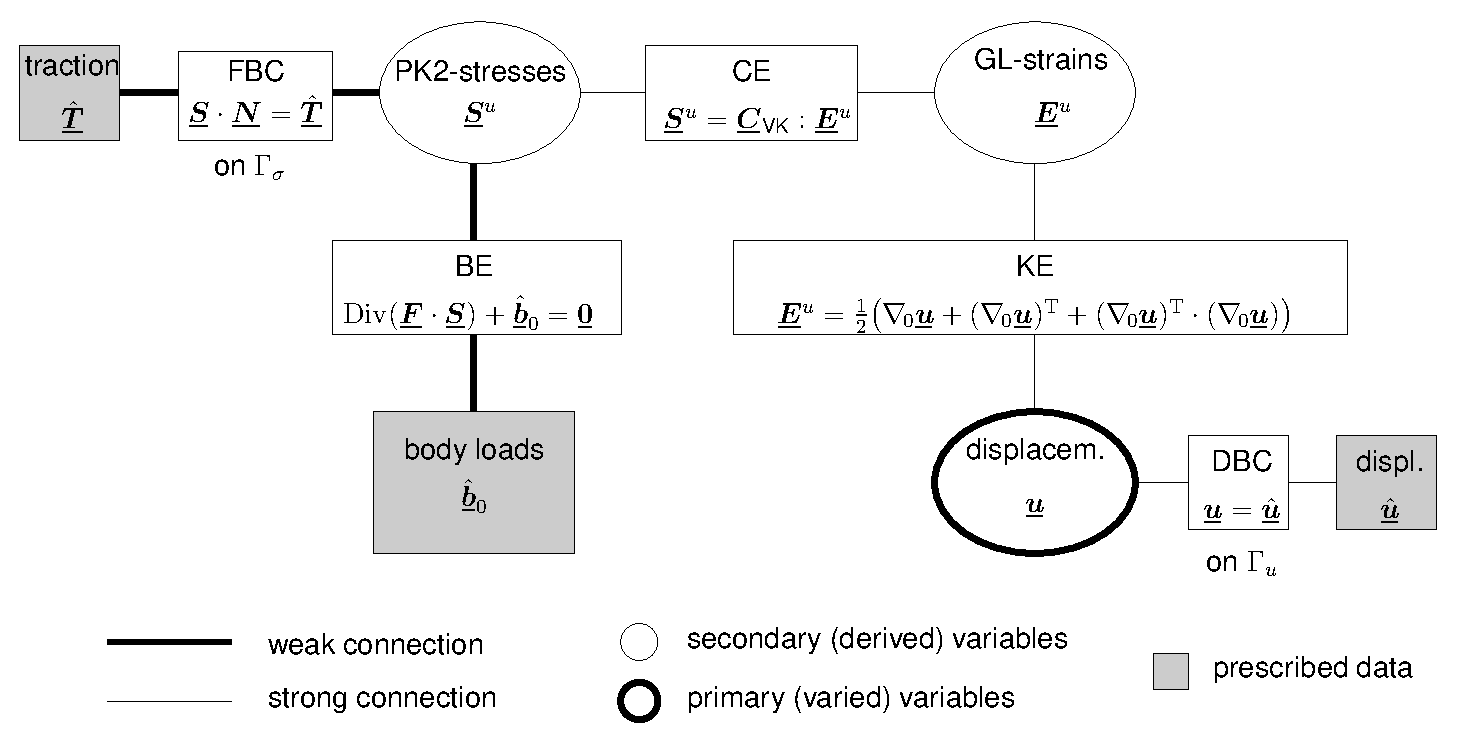
\includegraphics[width=\linewidth]{eps/tonti_nonlinear_elasto_statics}
\end{center}
\caption{Material description of displacement-based, static, geometrically
  nonlinear continuum mechanics}
\label{wall1:fig:tonti-nonlin}
\end{figure}

\subitempart{Balance equations (BE)}\\
The balance equations can be derived by considering an infinitesimal volume
element of the body. For
large deformations the equilibrium has to be enforced in the \emph{deformed}
state: $\ddiv \tns{\sigma}_\CT + \frac{\rho}{\rho_0} \hat{\tns{b}}_0 =
\vct{0}$. Throughout this chapter we deal with density-proportional body loads
($\rho_0$ density in undeformed/reference configuration; $\rho$ density in
deformed/current configuration; mass conservation). With
respect to the undeformed configuration this equilibrium reads 
\begin{equation}
\begin{array}{c}
\Ddiv \underbrace{\tns{P}}_{\tns{F} \cdot \tns{S}} + \;\;\hat{\tns{b}}_0 
= \vct{0}
\end{array}
\end{equation}
We use the 2nd Piola--Kirchhoff stresses $\tns{\sigma}_{\PK} =: \tns{S}$
and the work conjugate Green-Lagrange strains $\tns{\eps}_{\GL} =:
\vct{E}$, and get the following equilibrium equation.
\begin{equation}
\Ddiv( \tns{F} \cdot \tns{S} ) + \hat{\tns{b}}_0 = \tns{0}  
\qquad\text{in}\;\;\set{B}_0 = \Omega
\end{equation}


\subitempart{Kinematic equations (KE)} \\
The \name{Green}--\name{Lagrange} strain tensor was derived as:
\begin{equation}
  \tns{E} 
  = \tfrac{1}{2} \left ( \tns{F}^{\T} \cdot \tns{F} - \tns{1} \right ) 
  = \tfrac{1}{2} ( \underbrace{\Nabla \tns{u} + (\Nabla
  \tns{u})^\T}_{\text{linear part}} + \underbrace{(\Nabla \tns{u})^{\T}
  \cdot \Nabla \tns{u}}_{\text{nonlinear part}} )  
\end{equation}
The in-plane strains for a wall structure are given as:\\
\begin{equation}
\begin{aligned}
E_{11} & = u_{1,1} + \tfrac{1}{2} \Big( u_{1,1}^{2} + u_{2,1}^{2} \Big)
\\
E_{22} & = u_{2,2} + \tfrac{1}{2} \Big( u_{2,2}^{2} + u_{1,2}^{2} \Big)
\\
E_{12} & = \tfrac{1}{2} \Big( u_{1,2} + u_{2,1} + u_{1,1} u_{1,2} + u_{2,1}
  u_{2,2} \Big)
\\
E_{21} & = E_{12} \qquad \text{(symmetry)}
\end{aligned}
\end{equation}
The symmetry of $\tns{E}$ allows for writing the \name{Green}--\name{Lagrange}
strain vector with three relevant components
\begin{equation}
  \vct{E} 
  = \left[\begin{array}{c}
    E_{11} \\ E_{22} \\ \hdashline 2E_{12}
  \end{array}\right]
\end{equation}

\subitempart{Constitutive equations (CE)} \\
We assume linear-elastic behaviour, i.e.\@ we use the
\name{Saint~Venant}--\name{Kirchhoff} material model. 
\begin{equation}
  \tns{S} = \tns{C}_\VK : \tns{E} 
\end{equation}
The constitutive matrix $\vct{C}_\VK$ can be written in matrix notation
for a \emph{plane stress} 
state with the $X_{3}$-coordinate perpendicular on the
wall middle plane.\\
\begin{equation}
\begin{array}{cccc}
  \left [ \begin{array} {c} S_{11} \\ S_{22} \\\hdashline S_{12} \end{array}
  \right ] 
& = 
& \dfrac{E}{1 -\nu^{2}} \left [ \begin{array} {cc:c} 1 & \nu & 0
  \\ \nu & 1 & 0 \\ \hdashline 0 & 0 & \frac{1 -\nu}{2} \end{array} \right ] &
  \left [ 
  \begin{array} {c} E_{11} \\ E_{22} \\ \hdashline 2 E_{12} \end{array} \right ]
\\[4ex]
  \vct{S}
&
& \vct{C}_\text{VK} \, (\text{plane stress}) 
& \vct{E}
\end{array}
\end{equation}
This is the same plane stress constitutive matrix like in linear, planar
continuum mechanics.

\subitempart{Boundary conditions (BC)} \\
\begin{align}
&  \text{DBC}
&& \tns{u} = \hat{\tns{u}} 
&& \forall \vct{x} \in \Gamma_{u}
\\
&  \text{FBC}
&& \tns{P} \cdot \tns{N}
   = \hat{\tns{t}}_0 
   \quad\text{or}\quad
   \tns{S} \cdot \tns{N} = \hattns{T}
&& \forall \vct{x} \in \Gamma_{\sig}
\end{align}
using the normal on the undeformed boundary $\tns{N}$ and the pseudo traction
$\hat{\tns{T}} := \hat{\tilde{\tns{t}}} = \tns{F}^{-1} \hattns{t}_0$
(cf. Chap.~\ref{wall1:sec:noncon}). 


\subsection{Weak form}
For a FE-formulation we need the weak form of equilibrium. The pure displacement-based approach utilizes weighted
residuals of the balance equation and the traction boundary condition (FBC).  
\begin{equation}
  \delta W 
  = \int_{\Omega} \delta \tns{u} \cdot \underbrace{\Big[ \Ddiv \left (\tns{F}
    \cdot \tns{S} \right ) + \hat{\tns{b}}_0 \Big]}_{\text{residual of BE}}
    \dd V
  + \int_{\Gamma_\sig} \virt\tns{u} \cdot \underbrace{\Big[ \hattns{t}_{0} -
  \tns{F} \cdot \tns{S} \cdot \tns{N} \Big]}_{\text{residual of FBC}} \dd A
  = 0
\end{equation}

We already showed that Gauss' divergence theorem plus the appropriate boundary
conditions lead to the well-known principle of virtual work (PvW) expression:
\begin{equation}
  \delta W 
  = \underbrace{\int_{\Omega} \delta \tns{E} : \tns{S} \dd V}_{-\delta
 W_\Int} \;\; \underbrace{- \int_{\Omega} \delta \tns{u} \cdot \hat{\tns{b}}_0 \dd V
 - \int_{\Gamma_\sig} \delta \tns{u} \cdot \hat{\tns{t}}_0 \dd A}_{-\delta W_{\Ext}} =
 0 \qquad \qquad  \text{PvW}  
\end{equation}
with
\begin{align}
  \delta\tns{E} 
  & = \frac{\partial\tns{E}}{\partial\tns{F}} : \delta \tns{F}
  = \frac{1}{2} \Big[ \virt\tns{F}^{\T} \cdot \tns{F} + \tns{F}^{\T} \cdot
  \virt\tns{F} \Big] 
\\
  \delta \tns{E} : \tns{S} 
  & = \frac{1}{2} \Big[ \virt\tns{F}^{\T}
  \cdot \tns{F} + \tns{F}^{\T} \cdot \virt\tns{F} \Big] : \tns{S} 
  \;\underneath{=}{\text{symmetry of}\; \, \tns{S}}
  \big(\virt\tns{F}^{\T} \cdot \tns{F}\big) : \tns{S}
\end{align}
Keep in mind: $\tns{E}$ and therefore $\tns{S}$ depend \emph{nonlinearly} on
$\tns{u}$. 

%%
%%============================
\subsection{Discretization}
We focus on a discretization for a wall element with bi-linear shape functions
for the displacements. 

\subitempart{Displacement approach}\\
Within one element we get:

\begin{figure}[H]
   \begin{center}
%     \includegraphics[scale=1,angle=-90]{eps/ch6.3_1st.eps}
     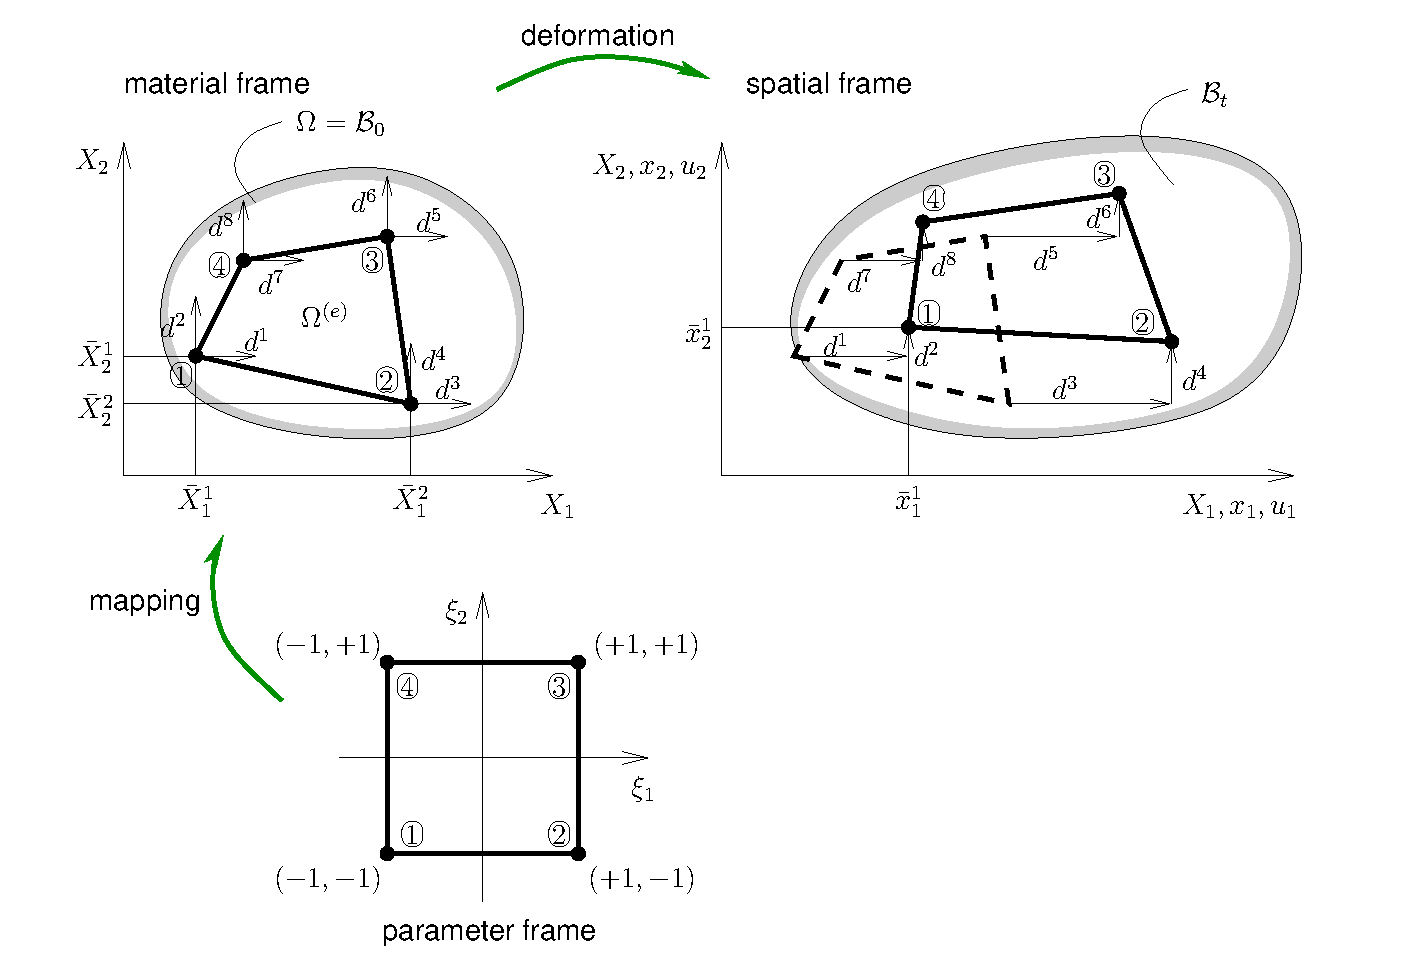
\includegraphics[width=0.8\linewidth]{eps/wall_element_and_mappings}
   \end{center}
\end{figure}

Here the nodal displacements $d^j$ ($j=1,\ldots,8$) are node by node $\tc{k}$
numbered displacements in 
$x_1$- and $x_2$-direction, i.e.\@ $u_i^k = d^{2k-2+i}$
(with $i=1,2$ and $k=1,\ldots,4$). 

The displacement approach appears as:\\
\begin{equation}
\begin{array}{cccc}
  \left [ \begin{array} {c} u_{1} \\ u_{2} \end{array} \right ]^{(e)} 
  & = &
   \left [ \begin{array} {cc:cc:cc:cc} N^{1} & 0 & N^{2} & 0 & N^{3} & 0 &
   N^{4} & 0 \\ 0 & N^{1} & 0 & N^{2} & 0 & N^{3} & 0 & N^{4} \end{array}
   \right ] &  \left [ \begin{array} {c} d^{1} \\ d^{2} \\ \hdashline d^{3} \\ d^{4}
  \\ \hdashline d^{5} \\ d^{6} \\ \hdashline d^{7} \\ d^{8} \end{array}
  \right]
\\
  \vct{u}^{(e)} (\xi_1,\xi_2) & = & \vct{N} (\xi_1,\xi_2) & \vct{d}
\end{array}
\end{equation}

and for the virtual displacements:\\
\begin{equation}
  \delta \vct{u}^{(e)} = \vct{N} \, \virt\vct{d}
\end{equation}

\begin{table}[H]
\begin{center}
\begin{tabular}{|c|c|c|} \hline
  $N^{k}$ & $N^{k}_{,\xi_1}$ & $N^{k}_{,\xi_2}$ 
\\ \hline
    $N^{1} = \frac{1}{4} (1-\xi_1) (1-\xi_2)$
  & $- \frac{1}{4} (1-\xi_2)$ & $- \frac{1}{4}(1-\xi_1)$ 
\\ \hline
    $N^{2} = \frac{1}{4} (1+\xi_1) (1-\xi_2)$ 
  & $\frac{1}{4} (1-\xi_2)$ & $- \frac{1}{4}(1+\xi_1)$ 
\\ \hline
    $N^{3} = \frac{1}{4} (1+\xi_1) (1+\xi_2)$ 
  & $\frac{1}{4} (1+\xi_2)$ & $\frac{1}{4}(1+\xi_1)$ 
\\ \hline
    $N^{4} = \frac{1}{4} (1-\xi_1) (1+\xi_2)$ 
  & $- \frac{1}{4} (1+\xi_2)$ & $\frac{1}{4}(1-\xi_1)$ 
\\ \hline
\end{tabular}
\end{center}
\caption{Bi-linear Lagrange-polynomials and their derivatives}
\end{table}

\subitempart{Geometry}

The geometry is discretized, according to the isoparametric concept:\\
\begin{equation}
\begin{aligned}
&  \vct{X}^{(e)} = \vct{N} \barvct{X}
&& \text{on}\;\;\Omega^{(e)}
\end{aligned}
\end{equation}

\subitempart{Discretized deformation gradient and other quantities}

The discrete deformation gradient takes the form
\begin{equation}
  \tns{F}^{(e)} 
  = \tns{1} + \frac{\partial\tns{u}^{(e)}}{\partial\tns{X}}
  = \left[\begin{array}{cc}
       1 & 0
    \\ 0 & 1
    \end{array}\right]
  + \left[\begin{array}{cc}
       \frac{\pd u_1}{\pd X_1} & \frac{\pd u_1}{\pd X_2}
    \\ \frac{\pd u_2}{\pd X_1} & \frac{\pd u_2}{\pd X_2}
     \end{array}\right]^{(e)}
\end{equation}

In matrix notation it is useful to write it either as a vector or a
 matrix. For a vector notation $\tns{F}$ can be arranged like\\
\begin{equation}
\begin{array}{ccccc}
 \tilde{\vct{F}}^{(e)} 
 =  \left[ \begin{array}{c} 
     F_{11} \\ F_{22} \\ F_{12} \\ F_{21} 
    \end{array} \right] 
& = \left[ \begin{array} {c} 1 \\ 1 \\ 0 \\
0 \end{array} \right] & + \underbrace{\left[ \begin{array} {cc} \partial_{X_{1}} & 0 \\ 0 &
 \partial_{X_{2}} \\ \partial_{X_{2}} & 0 \\ 0 & \partial_{X_{1}} \end{array}
 \right ]} & \left[ \begin{array} {c} u_{1} \\ u_{2}
 \end{array} \right ]^{(e)} & \begin{array} {r} = : \tilde{\vct{H}} \\ = :
 \tilde{\vct{1}} + \overbrace{\underbrace{\vct{L} \vct{N}} \vct{d}} \\
 =:\vct{B}_\text{L} \end{array} \\
& \quad \tilde{\vct{1}} & = : \vct{L} & & \\
\end{array} 
\end{equation}
(Remember: $\tns{F}$ is not symmetric!)
We will use as well a matrix notation of $\tns{F}$ in the form:
\begin{equation}
\begin{array}{ccc}
\bar{\mat{F}}^{(e)} 
= \left [ \begin{array} {ccc}  
     F_{11} & 0 & F_{12}
  \\ 0 & F_{22} & F_{21}
  \\ 0 & F_{12} & F_{11} 
  \\ F_{21} & 0 & F_{22}
  \end{array} \right ] 
& = \left [ \begin{array} {ccc}  
     1 & 0 & 0
  \\ 0 & 1 & 0
  \\ 0 & 0 & 1 
  \\ 0 & 0 & 1
  \end{array} \right ] 
& + \left [ \begin{array} {ccc}  
     H_{11} & 0 & H_{12} 
  \\ 0 & H_{22} & H_{21} 
  \\ 0 & H_{12} & H_{11} 
  \\ H_{21} & 0 & H_{22}
  \end{array} \right ] \\[5ex]
& \bar{\vct{1}} & \bar{\vct{H}}
\end{array} 
\end{equation}
in which $H_{ij}$ are the components of the displacement gradient vector\\
$\tilde{\vct{H}} = 
\begin{bmatrix} H_{11} & H_{22} & H_{12} & H_{21} \end{bmatrix}^\T = \mat{L}
\mat{N} \vct{d} = \mat{B}_\text{L} \vct{d}$. 


The $\mat{B}_\text{L}$ matrix
is constructed as follows: We see a linear dependence of $\tns{F}^{(e)}$ on
$\tns{u}^{(e)}$: 
\begin{equation}
\begin{array}{ccc}
\dfrac{\partial \tilde{\vct{F}}}{\partial\vct{d}} = \vct{B}_\text{L} & \text{with}
& \vct{B}_\text{L} = \vct{L} \vct{N} = \left [ \begin{array} {cc:cc:cc:cc}
    N^{1}_{,X_{1}} & 0 & N^{2}_{,X_{1}} & 0 & N^{3}_{,X_{1}} & 0 & N^{4}_{,X_{1}} & 0 \\ 0
    & N^{1}_{,X_{2}} & 0 & N^{2}_{,X_{2}} & 0 & N^{3}_{,X_{2}} & 0 & N^{4}_{,X_{2}} \\
    N^{1}_{,X_{2}} & 0 & N^{2}_{,X_{2}} & 0 & N^{3}_{,X_{2}} & 0 & N^{4}_{,X_{2}} & 0 \\ 0
    & N^{1}_{,X_{1}} & 0 & N^{2}_{,X_{1}} & 0 & N^{3}_{,X_{1}} & 0 & N^{4}_{,X_{1}}
  \end{array} \right ]
\end{array} 
\end{equation}

The element is defined on the element parameter domain
$\{\vct{\xi} \forwhich \vct{\xi} \in  [-1,+1]\times[-1,+1]\}$ and all
quantities are referred back to this parameter space, in particular, the shape
functions. Therefore, differentiations with respect to the material
coordinates $\vct{X}$ have to be expressed as differentiations with respect to
$\vct{\xi}$. In essence, the isoparametric concept enables conveniently this.

For the evaluation of derivatives with respect to the material coordinates
$\vct{X}$, the Jacobian matrix is used:\\
\begin{equation}
  \left[ \begin{array} {r} \partial_{X_{1}} (\cdot) \\ \partial_{X_{2}} (\cdot) \end{array}
  \right ] = \vct{J}^{-1} \left [ \begin{array} {c} \partial_{\xi_1} (\cdot) \\
  \partial_{\xi_2} (\cdot) \end{array} \right ]
\end{equation}

with, evaluated at $(\xi_1,\xi_2)$,
\begin{equation}
  \vct{J}^{-1} 
  = \frac{1}{\det \vct{J}} \left [ \begin{array}
  {rr}  \frac{\partial X_{2}}{\partial \xi_2} & - \frac{\partial
  X_{2}}{\partial \xi_1} \\[1ex] - \frac{\partial X_{1}}{\partial \xi_2} &
  \frac{\partial X_{1}}{\partial \xi_1} \end{array} \right ]
  \qquad\text{and}\qquad
  \det \vct{J} =
  \frac{\partial X_{1}}{\partial \xi_1} \frac{\partial X_{2}}{\partial \xi_2} -
  \frac{\partial X_{1}}{\partial \xi_2} \frac{\partial X_{2}}{\partial \xi_1} 
  \period
\end{equation}
Here, the material derivatives are obtained by introducing the isoparametric
concept\\
\begin{equation}
  \left[\begin{array}{c} 
      \frac{\pd X_1^{(e)}}{\pd \xi_\alpha} \\ \frac{\pd X_2^{(e)}}{\pd \xi_\alpha}
  \end{array}\right]
  = \mat{N}_{,\xi_\alpha} \barvct{X}
  \qquad\text{on}\;\;\Omega^{(e)}\quad\text{with}\;\;\alpha=1,2
  \period
\end{equation}

Finally, the isoparametric Jacobian is summarized as follows:
\begin{equation}
  \mat{J}
  = \begin{bmatrix}
    \frac{\pd X_1}{\pd \xi_1}  &  \frac{\pd X_2}{\pd \xi_1}
  \\
    \frac{\pd X_1}{\pd \xi_2}  &  \frac{\pd X_2}{\pd \xi_2}
  \end{bmatrix}
  = \left[\begin{array}{c}
    \big( \mat{N}_{,\xi_1} \barvct{X} \big)^\T
  \\
    \big( \mat{N}_{,\xi_2} \barvct{X} \big)^\T
  \end{array}\right]
  \period
\end{equation}


\subitempart{Assembly of global system of nonlinear equilibrium equations}\\
The integrals in the PVW are evaluated by the appropriate integrals within the
individual elements which then are assembled in the usual way. The unknown
nodal displacements of the whole system (DOFs) are then called $\vct{D}$.

Firstly, the integration on the domain $\Omega$ --- the undeformed body domain
--- is  carried out element-wise on each element domain $\Omega^{(e)}$
\begin{equation}
  \int_{\Omega} (\cdot) \, \dd V 
  = \sum_{e=1}^{\nele} \int_{\Omega^{(e)}} (\cdot) \, \dd V
  \period
\end{equation}
(Strictly, the equal sign might be replaced by `$\approx$' as the elements
may not cover the complete original domain $\Omega$. For instance, this occurs
if $\Omega\subset\R^2$ has \emph{curved} boundaries and is discretised with
bi-linear quadrilaterals. The curved boundaries cannot be exactly recovered
with bi-linear quadrilaterals; they always have a polygonal boundary.)

Consequently, the internal and external virtual work becomes per element
\begin{align}
& -\virt W_\Int^{(e)}
  = \int_{\Omega^{(e)}} \virt\tns{E} : \tns{S} \, \dd V
  \comma
&& \virt W_\Ext^{(e)}
  = \int_{\Omega^{(e)}} \virt \tns{u} \cdot \hattns{b}_0 \, \dd V
  + \int_{\Gamma_{\sig}^{(e)}} \virt\tns{u} \cdot \hattns{t}_0 \, \dd A
  \period
\end{align}

The discrete version of $\virt\tns{E} : \tns{S}$ within is given as
\begin{equation}
\begin{array}{lc}
  \text{starting from} \qquad 
& \delta \tns{E}^{(e)} 
  = \frac{1}{2} \left [\delta \tns{F}^{(e)\T} \tns{F}^{(e)} 
  + \tns{F}^{(e)\T} \delta \tns{F}^{(e)} \right ] \\
& 
\\
  \text{in matrix notation:} \qquad 
& \delta \vct{E}^{(e)} 
  = \underbrace{\bar{\vct{F}}^{(e)\T} \left (\vct{B}_\text{L} \delta \vct{d}
  \right )} \\
& \text{symmetric, induced by the arrangement of} \,\bar{\vct{F}}^{(e)} 
\end{array} 
\end{equation}
The scalar product $\delta \tns{E}^{(e)} : \tns{S}^{(e)}$ in matrix-notation
reads 
\begin{equation}
  (\delta \vct{E}^{(e)})^{\T} \vct{S}^{(e)} 
  = \delta \vct{d}^{\T}
  (\vct{B}_\text{L}^{\T} \bar{\vct{F}}^{(e)})  \vct{S}^{(e)}
\end{equation}
Hence, the element, discrete, internal virtual work can be written\\
\begin{equation}
   -\virt W_\Int^{(e)}
   = \virt\vct{d}^\T \int_{\Omega^{(e)}} 
   \mat{B}_\text{L}^\T \, \barmat{F} \, \vct{S}
   \,  \dd V
\end{equation}

We arrive at the discrete version of the PVW\\
\begin{equation}
\begin{array}{rrcccr}
   \delta W =
&  \delta \vct{D}^{\T} \displaystyle\Ass{e=1}{\nele} \Bigg[
&  \underbrace{\int_{\Omega^{(e)}} \vct{B}_\text{L}^{\T} \bar{\vct{F}}
   \vct{S} \dd V}_{\vct{f}_\Int^{(e)}(\vct{d})}
&  -
&  \underbrace{\Big(\int_{\Omega^{(e)}} \vct{N}^{\T}
   \hat{\vct{b}}_0 \dd V + \int_{\Gamma_{\sig}^{(e)}} \vct{N}^{\T}
   \hat{\vct{t}}_0  \dd A\Big)}_{\vct{f}_\Ext^{(e)}(\lambda)}
&  \Bigg] = 0
\\[6ex]
   \Longrightarrow
&  
&  \underbrace{\displaystyle\Ass{e=1}{\nele} \vct{f}_\Int^{(e)}(\vct{d})}_{\displaystyle\vct{F}_\Int(\vct{D})}
&  -
&  \underbrace{\displaystyle\Ass{e=1}{\nele} \vct{f}_\Ext^{(e)}(\lambda)}_{\displaystyle\vct{F}_\Ext(\lambda)}
&  = \vct{0}
\end{array}
\end{equation}



This is the \emph{discrete nonlinear} equation to be solved at certain load
levels by  Newton--Raphson iterations for instance. Therefore, we need a
linearized form of
\begin{equation}
  \vct{R} 
  = \vct{F}_{\Int}(\vct{D}) - \vct{F}_{\Ext} 
  = \vct{0}
  \period
\end{equation}

%%
%%============================
\subsection{Linearization}
The linearization around a displacement state reads at the $(k+1)$th increment and
at the $i$th iteration $\vct{D}_{k+1}^{i} = : \vct{D}^{i}$:
\begin{equation}
\begin{array}{ll}
\multicolumn{2}{r}{\qquad \qquad \qquad \qquad \qquad \qquad \text{incremental
    unknown nodal displacements}} \\ 
\Lin \vct{R} = \underbrace{\vct{R} (\vct{D}^{i})} +
\underbrace{\left.\frac{\partial \vct{R} (\vct{D})}{\partial \vct{D}}
  \right|_{\vct{D}^{i}}} \overbrace{\Delta \vct{D}^{i+1}} = \vct{0} & \\
\multicolumn{2}{l}{\qquad \text{``RHS''-term} \qquad \text{tangential
stiffness} \, \vct{K}_\text{T}}  
\end{array} 
\end{equation}
in which RHS abbreviates right-hand-side.

Or in terms of assembled quantities
\begin{equation}
\begin{split}
   \Lin \vct{R} = \vct{R} (\vct{D}^{i}) 
   + \Ass{e=1}{\nele} \Bigg[
&  \int_{\Omega^{(e)}} \left ( (\vct{B}_\text{L}^{\T} \bar{\vct{F}}^{i})
   \; \vct{S}_{,\vct{d}}^{i} \;+\; (\vct{B}_\text{L}^{\T}
   \bar{\vct{F}}^{i})_{,\vct{d}} \; \vct{S}^{i} \right ) \dd V 
\\
&  - \int_{\Omega^{(e)}} \mat{N}^\T \hatvct{b}_{0\;,\vct{d}} \, \dd V
   - \int_{\Gamma_{\sig}^{(e)}} \left ( \vct{N}^{\T}
  \hat{\vct{t}}_{0\;,\vct{d}} 
\right ) \dd A \Bigg ]^{(e)} \Delta \vct{D}^{i+1} = \vct{0}
\end{split}
\end{equation}



\subitempart{Deformation-independent load}\\
If we restrict ourselves to deformation-independent load
cases, then we obtain  $\hat{\vct{b}}_{0\;,\vct{d}} = \vct{0}$ \emph{and}
$\hat{\vct{t}}_{0\;,\vct{d}} = \vct{0}$. The linearized balance equations
simplify due to the cancelled terms: 
\begin{equation}
  \Lin \vct{R}
  = \vct{R} (\vct{D}^{i})  
  + \displaystyle\Ass{e=1}{\nele} \Bigg[ \int_{\Omega^{(e)}} \Big( 
  \underneath[3ex]{\underbrace{(\vct{B}_\text{L}^{\T} \bar{\vct{F}}^{i})
  \vct{S}_{, \vct{d}}^{i}}}{\text{elastic and initial displacement stiffness $\mat{k}_\text{e}^{(e)} + \mat{k}_\text{u}^{i(e)}$}}
  + \underneath{\underbrace{( \vct{B}_\text{L}^{\T}
  \bar{\vct{F}}^{i})_{,\vct{d}}\vct{S}^{i}}}{\text{geometric stiffness $\mat{k}_\text{g}^{i(e)}$}}
  \Big) \dd V \Bigg]^{(e)} \Delta \vct{D}^{i+1} 
  = \vct{0}
\end{equation}

%%
%%----------------------------
\subsubsection{Elastic and initial displacement stiffness matrices}
The elastic and initial displacement stiffness matrices are\\
\begin{equation}
  \vct{k}_\text{eu}^{i(e)} 
  = \int_{\Omega^{(e)}} ( \vct{B}_\text{L}^{\T}
\bar{\vct{F}}^{i} ) \vct{S}_{,\vct{d}}^{i} \dd V
\end{equation}
with
\begin{equation}
  \vct{S} = \vct{C}_\VK \vct{E}
\end{equation}
and from
\begin{align}
  \tns{E}
& = \frac{1}{2} \left [ \tns{F}^{\T} \cdot \tns{F} -
  \tns{1} \right ]
&&\text{we get the vector}
& \vct{E}
& =\frac{1}{2} \left [ (\barmat{F})^{\T} \tildevct{F} - \tilde{\vct{1}}
  \right ]
\end{align}
as well as
\begin{equation}
  \tns{E}_{, \vct{d}} = \frac{1}{2} \left [ \tns{F}_{,
    \vct{d}}^{\T} \cdot \tns{F} + \tns{F}^{\T} \cdot \tns{F}_{, \vct{d}} \right
]
\qquad\text{in matrix notation}\qquad
\vct{E}_{,\vct{d}}
= \barmat{F}^{\T} \tildevct{F}_{,\vct{d}} 
= \bar{\vct{F}}^{\T} \vct{B}_\text{L}
\end{equation}
So we end up with
\begin{equation}
  \leadsto\qquad 
  \vct{S}_{, \vct{d}}^{i} 
  = \vct{C}_\VK \vct{E}_{,\vct{d}}^{i} 
  = \vct{C}_\VK ( \bar{\vct{F}}^{i})^{\T} \vct{B}_\text{L}
\end{equation}

We achieve the following expression\\
% \begin{equation*}
%    \hspace{-3cm}
%    \mat{k}_\text{eu}^{i(e)} 
%    = \int_{\Omega^{(e)}} \underneath{\underbrace{\mat{B}_\text{L}^{\T}
%      \overneath{\overbrace{\Big( \bar{\mat{F}}^{i} \mat{C}_\VK
%    \bar{\mat{F}}^{i\T} \Big)}}{\text{constitutive matrix mapped to the current
%    configuration}}}}{\text{$=\mat{B}^{i\T}\mat{C}_\VK \mat{B}^i$ with
%    nonlinear $\mat{B}^i := (\mat{F}^i)^\T \mat{B}_\text{L}$}}
%      \mat{B}_\text{L}^{\T} \, \dd V
% \end{equation*}
\begin{equation}
\begin{array}{lccc}
& \multicolumn{2}{l}{\text{constitutive matrix mapped to the current
    configuration}} & \\
& & & \\
\multicolumn{2}{l}{\Longrightarrow\quad \vct{k}_\text{eu}^{i(e)} = \displaystyle\int_{\Omega^{(e)}}
  \underbrace{\vct{B}_\text{L}^{\T} \overbrace{ \left ( \bar{\vct{F}}^{i} \mat{C}_\VK
  \bar{\vct{F}}^{i^{\T}} \right )}\vct{B}_\text{L}}  \, \dd V} & & \\
& & & \\[6ex]
& \multicolumn{2}{l}{\qquad \qquad = \vct{B}^{i\T} \mat{C}_\VK \vct{B}^{i} \, \text{with a
    nonlinear} \, \vct{B}^{i} := (\barmat{F}^{i})^{\T} \vct{B}_\text{L}} & 
\end{array} 
\end{equation}

This element stiffness can be split in a purely elastic, deformation
independent stiffness $\vct{k}_\text{e}^{(e)}$ (the same as for a geometric
linear analysis) and a stiffness $\vct{k}_\text{u}^{(e)i}$ due to the initial
deformation $\vct{d}^{i}$.
\begin{equation}
\begin{split}
    \vct{k}_\text{eu}^{i(e)}
&   = \int_{\Omega^{(e)}} \vct{B}_\text{L}^{\T} \left (
    (\bar{\vct{1}} + \bar{\vct{H}}^{i}) \, \vct{C}_\VK \, ( \bar{\vct{1}} +
\bar{\vct{H}}^{i} )^{\T} \right ) \vct{B}_\text{L} \dd V 
\\ 
&  = \underbrace{\int_{\Omega^{(e)}} 
     (\overbrace{\barmat{1}^\T\vct{B}_\text{L}}^{\mat{B}_\text{lin}})^{\T} 
     \vct{C}_\VK
     \overbrace{\barmat{1}^\T \vct{B}_\text{L}}^{\mat{B}_\text{lin}}
     \dd V}_{\displaystyle \mat{k}_\text{e}^{(e)}}  
\\
&   \quad  + \underbrace{
    \int_{\Omega^{(e)}} \left[ 
      \vct{B}_\text{L}^{\T} \left(
        \barmat{1} \, \vct{C}_\VK \, \bar{\vct{H}}^{i\T} 
      \right) \vct{B}_\text{L} 
    + \vct{B}_\text{L}^{\T} \left(
        \bar{\vct{H}}^{i} \, \vct{C}_\VK  \, \barmat{1}^\T
      \right) \vct{B}_\text{L} 
    + \vct{B}_\text{L}^{\T} \left( 
        \bar{\vct{H}}^{i} \vct{C}_\VK \bar{\vct{H}}^{i\T} 
      \right) \vct{B}_\text{L} 
    \right] \dd V}_{\displaystyle \mat{k}_\text{u}^{i(e)}}
\end{split}
\end{equation}
Here, $\mat{B}_\text{lin}$ is the B-operator matrix occurring in the
geometrically linear FE-method (cf.\@ course ``Finite Elemente''):
\begin{equation}
  \mat{B}_\text{lin}
  = \barmat{1}^\T \mat{B}_\text{L}
  = \left[\begin{array}{cc:cc:cc:cc}
     N_{,X_1}^1 & 0  & N_{,X_1}^2 & 0  & N_{,X_1}^3 & 0  & N_{,X_1}^4 & 0 
  \\
     0 & N_{,X_2}^1 &  0 & N_{,X_2}^2 &  0 & N_{,X_2}^3  & 0 & N_{,X_2}^4
  \\
    N_{,X_2}^1  & N_{,X_1}^1  &  N_{,X_2}^2 & N_{,X_1}^2 &  N_{,X_2}^3 & N_{,X_1}^3 &  N_{,X_2}^4 & N_{,X_1}^4
  \end{array}\right]
\end{equation}

%%
%%----------------------------
\subsubsection{Geometric stiffness matrix}
The geometric element stiffness matrix can be written in a different way:\\
\begin{equation}
\vct{k}_\text{g}^{(e)}(\vct{d}^i) 
= \int_{\Omega^{(e)}} (\vct{B}_\text{L}^{\T}
\bar{\vct{F}}^{i} )_{,\vct{d}} \vct{S}^{i} \dd V 
= \int_{\Omega^{(e)}} \vct{B}_\text{L}^{\T} \bar{\vct{S}}^{i}
\vct{B}_\text{L} \dd V 
\end{equation}

Here for this matrix notation the stresses $\tns{S}$ are arranged as:\\
\begin{equation}
\barmat{S} = \left [ \begin{array} {cccc}  S_{11} & 0 & S_{12} & 0 \\
    0 & S_{22} & 0 & S_{12} \\ S_{12} & 0 & S_{22} & 0 \\ 0 & S_{12} & 0 &
    S_{11} \end{array} \right ]
\end{equation}

%%
%%----------------------------
\subsubsection{External and internal forces}\label{wall1:sec:wall-extforce}
The terms on the right hand side are given by
\begin{equation}
\vct{R} (\vct{D}^{i}) 
  = \Ass{e=1}{\nele} \Bigg[ \underbrace{\int_{\Omega^{(e)}}
  (\vct{B}_\text{L}^{\T} \bar{\vct{F}}^{i}) \vct{S}^{i} \,\dd
  V}_{\vct{f}_\Int^i} - \underbrace{\Big(\int_{\Omega^{(e)}} \vct{N}^{\T}
  \hat{\vct{b}}_0 \,\dd V + \int_{\Gamma_\sig^{(e)}} \vct{N}^{\T} \hat{\vct{t}}_0 \dd
  A \Big)}_{\vct{f}_\Ext}  \Bigg]
\end{equation} 

The first part describes the internal forces, which depend on the current
stresses and deformations; the second part, the external forces driven by
prescribed body and surface loads. The evaluation of the external forces is
the same as in linear analysis
\begin{equation}
\text{with body forces}\quad
\hatvct{b}_0 = \begin{bmatrix} \hat{b}_{0;1}(\vct{\xi})
               \\ \hat{b}_{0;2}(\vct{\xi}) \end{bmatrix}
\qquad\text{and surface loads}\qquad
\hatvct{t}_0 = \begin{bmatrix} \hat{t}_{0;1}(\vct{\xi})
               \\ \hat{t}_{0;2}(\vct{\xi}) \end{bmatrix}
\end{equation}

%%
%%---------------------------Q1E4
\section{Theory behind the enhanced assumed strain (EAS) wall element
(Q1E4) for geometrically non-linear analyses}\label{wall1:sec:walleas}

\begin{flushright}
  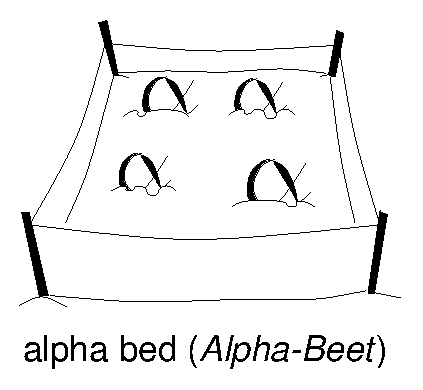
\includegraphics[width=0.2\linewidth]{eps/eas-alphabed}
\end{flushright}

%%
%%============================
\subsection{Motivation}
In courses about linear finite elements (e.g.\@ the course ``Finite
Elemente'') \intro{locking} phenomena are usually discussed. Locking was
qualitatively summarized as:
\begin{quote}
 \emph{locking is deterioration of convergence with respect to
one parameter}
\end{quote} (cf.\@ ``Finite Elemente''). 

For instance, plain, geometrically linear, $4$-node, bi-linear quadrilateral
wall elements 
exhibit \intro{shear locking} in bending situations and \intro{volumetric
locking} 
close to the incompressible limit ($\nu\to\frac{1}{2}$). The element
introduced in Section~\ref{wall1:sec:wall} is a geometrically nonlinear element, however, it must
recover of course the geometrically linear element in the case of small
deformations. Thus it is ridden by locking in the same way. 

In ``Finite Elemente'' shear locking was studied using the purely
displacement-based Q1 and the \name{Pian}--\name{Sumihara} wall element. The
\name{Pian}--\name{Sumihara} wall element is a mixed-hybrid element which
utilizes a \name{Hellinger}--\name{Reissner} two-field approach to circumvent
locking. 

\subpart{Let us repeat a paragraph of the ``Finite Elemente'' lecture notes:}\\
In the first example we investigate the convergence behaviour for a cantilever
with an end force. The configuration along with the analytical solution is
given in Figure~\ref{wall1:fig:eas-cwef}\@. Figure~\ref{wall1:fig:eas-cdfed} gives the
convergence behaviour for 
end displacements of the cantilever both for the \name{Pian}--\name{Sumihara}
element (P--S) and 
the ordinary bi-linear displacement element (Q1).  In this diagram $60$ DOFs
correspond to a $2\times10$ element mesh, $120$ DOFs to a $2\times20$ mesh and
$400$  DOFs to a 
$4\times40$ mesh, respectively. The latter mesh is also shown in
Figure~\ref{wall1:fig:eas-cwef}. The superior behaviour of the
\name{Pian}--\name{Sumihara} element as 
compared to the pure displacement element is rather obvious from this
diagram. The reason for this is the pronounced locking effect that is present
in the displacement formulation.

\begin{figure}[H]
\begin{multicols}{2}
\begin{flushleft}
    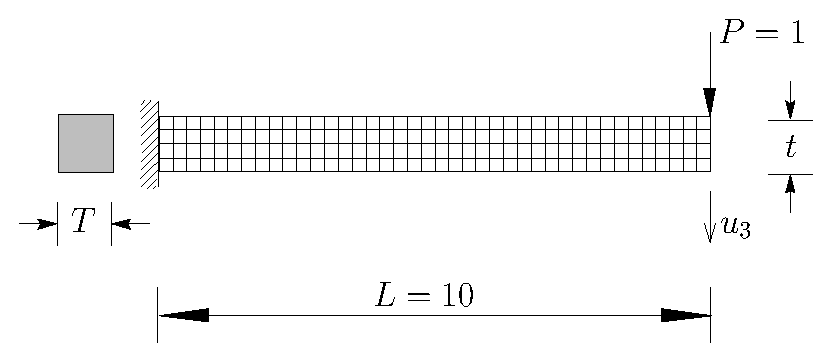
\includegraphics[width=0.9\linewidth]{eps/cantilever-with-end-force_b}
\end{flushleft}
\columnbreak

\begin{tabular}{lcl}
  $T=1$;  $t=1$  & & section modulus: 
\\
  $E=4\EE{6}$; $\nu=0$ & & $W=\frac{T t^{2}}{6}$
\end{tabular}
\vspace*{1.ex}

beam solution:\\
$u_{3,\text{exact}} = u_{3} = \frac{P L^{3}}{3EI} = 10^{-3}$ \\
$\sigma_{\text{max}} = \frac{PL}{W} = 60$
\end{multicols}
  \caption{Cantilever with end force: geometry, loads %
           and analytic beam solution}
  \label{wall1:fig:eas-cwef}
\end{figure}

\begin{figure}[H]
   \begin{center}
     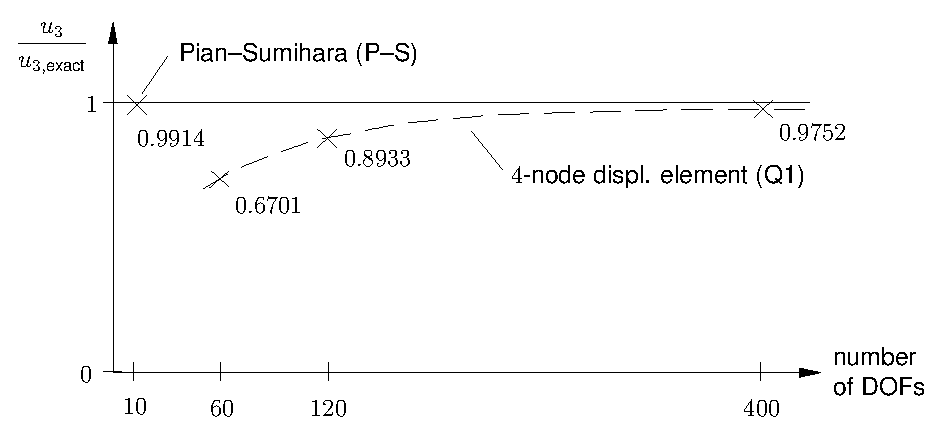
\includegraphics[width=0.9\textwidth]{eps/convergence-diagram-for-end-displacements}
   \end{center}
  \caption{Convergence diagram for end displacements}
 \label{wall1:fig:eas-cdfed}
\end{figure}


In ``Finite Elemente'' several approaches were introduced to circumvent
locking for linear problems.
\begin{itemize}
\item reduced integration ($\to$ often trouble with zero-energy-modes)
\item ``assumed natural strain'' (ANS) approaches ($\to$ $\barmat{B}$-matrix)
\item mixed elements ($\to$ based on multi-field functionals)
\end{itemize}

%%
%%============================
\subsection{Strong form}
The \name{Tonti}-diagram Figure~\ref{wall1:fig:tonti-nonlin-fp-pair} depicts the
boundary value problem which models 
static, geometrically nonlinear continuum mechanics particularizing in
\name{St.~Venant}--\name{Kirchhoff}'s  material.

\begin{figure}[H]
\begin{center}
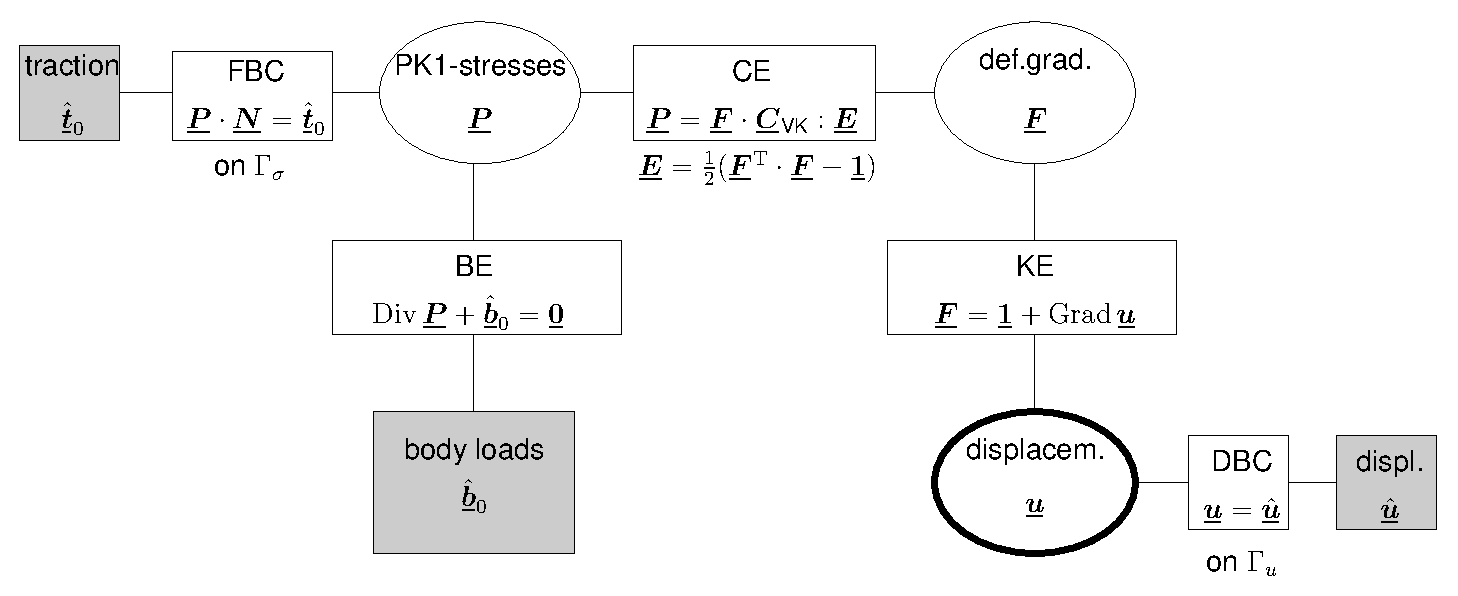
\includegraphics[width=\linewidth]{eps/tonti_nonlinear_elasto_statics_fp_pair}
\end{center}
\caption{Material description of displacement-based, static, geometrically
  nonlinear continuum mechanics}
\label{wall1:fig:tonti-nonlin-fp-pair}
\end{figure}

In Fig.~\ref{wall1:fig:tonti-nonlin-fp-pair} the energy-conjugate pair
material deformation gradient $\tns{F}$ and 1st \name{Piola}--\name{Kirchhoff}
stress 
$\tns{P}$ are applied. From a continuum mechanics viewpoint this is absolutely
equivalent to the form displayed in
Fig.~\ref{wall1:fig:tonti-nonlin} employing the pair $\tns{E}$ and $\tns{S}$. 



%%
%%============================
\subsection{The \name{Hu-Washizu} principle}
The \intro{\name{Hu-Washizu} principle} is a \intro{three-field
principle}. The term 
three-field principle stems from not only considering the displacements
$\tns{u}$ as an independent field variable but taking the deformation gradient
and the 1st \name{Piola}--\name{Kirchhoff} stress as well. So, we end up
formally with three primary variables/fields: $\tns{u}$, $\tns{F}$ and
$\tns{P}$. These 
are shown in Fig.~\ref{wall1:fig:tonti-hu-washizu-weak-form} together with the 
derived/secondary fields $\tns{F}^u$ and $\tns{P}^F$. These are connected by
the kinematic equations (KE) and constitutive equations (CE), respectively, to
their primary variables indicated by their superscript. 

% \begin{figure}[H]
% \begin{center}
% \includegraphics[width=\linewidth]{eps/tonti_hu_washizu_fp_pair_strong_form}
% \end{center}
% \caption{Three-field functional}
% \label{wall1:fig:tonti-hu-washizu-strong-form}
% \end{figure}

\begin{figure}[H]
\begin{center}
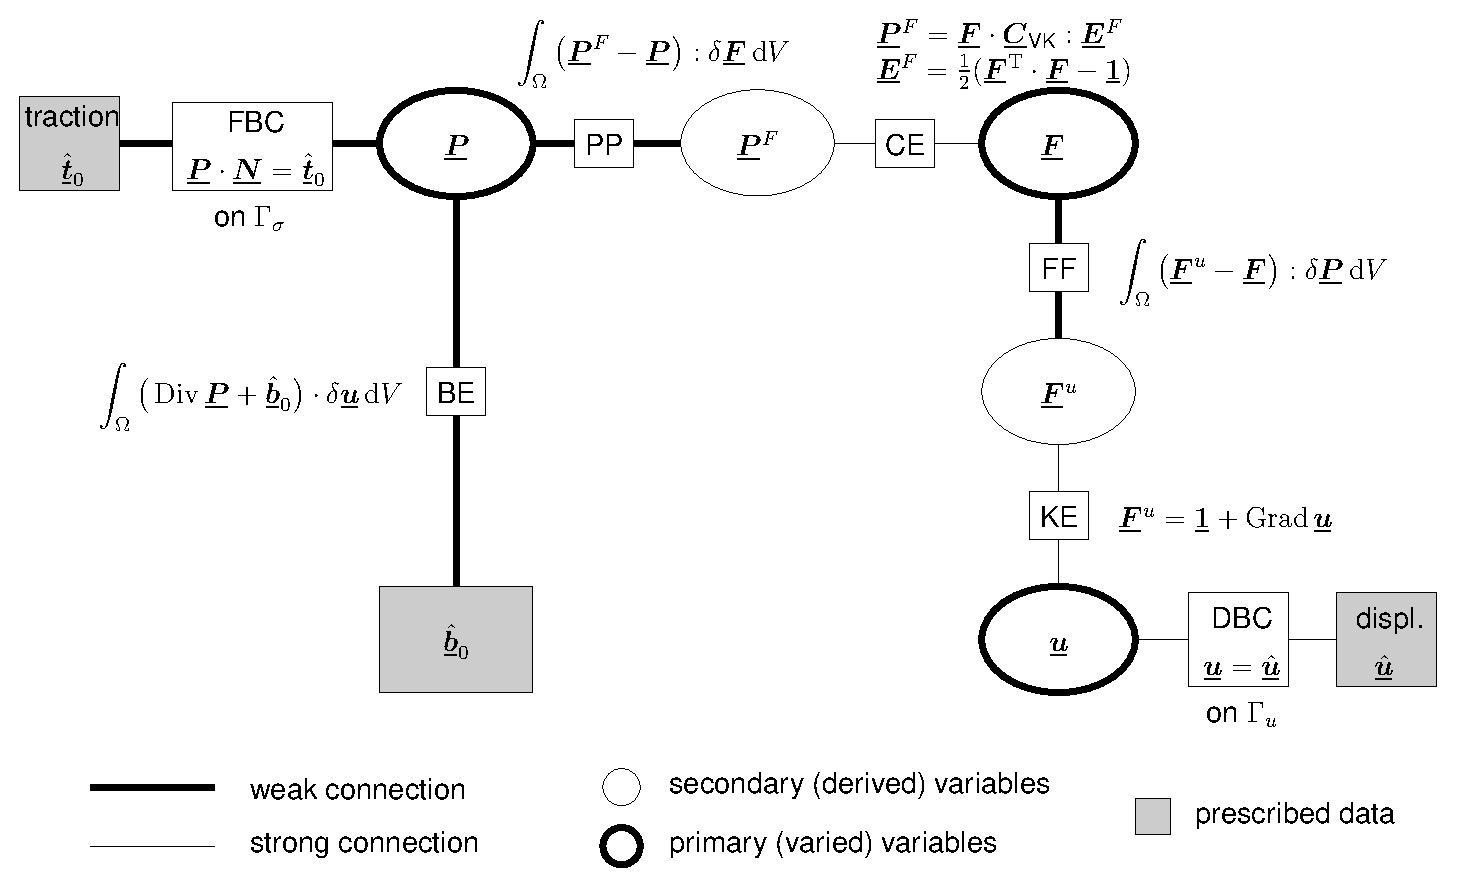
\includegraphics[width=\linewidth]{eps/tonti_hu_washizu_fp_pair_weak_form}
\end{center}
\caption{\name{Tonti}-diagram for \name{Hu-Washizu} principle}
\label{wall1:fig:tonti-hu-washizu-weak-form}
\end{figure}

The connections FF and PP define the residuals of the primary and secondary
deformation gradient and 1st \name{Piola}--\name{Kirchhoff} stress:
\begin{align}
  \text{FF :} \qquad
& \tns{R}_\FFF = \tns{F}^u - \tns{F} = \tns{0}
  \qquad \text{in $\Omega$}
\\
  \text{PP :} \qquad
& \tns{R}_\PPP = \tns{P}^F - \tns{P} = \tns{0}
  \qquad \text{in $\Omega$}
\end{align}

These residuals and the balance equation (BE) are weighted on the undeformed
domain $\set{B}_0 = \Omega$ by test functions. These test functions can be 
identified through work pairing as virtual counterparts of the primary
fields.
These weighted residuals have to vanish for any permissible test function; we
achieve
\begin{equation}
\begin{split}
  \virt \Pi_\HW 
& = \int_\Omega \overbrace{\big( \tns{F}^u - \tns{F} \big)}^{\tns{R}_\FFF} 
    : \virt\tns{P} \, \dd V
  + \int_\Omega \overbrace{\big( \tns{P}^F - \tns{P} \big)}^{\tns{R}_\PPP}
    : \virt\tns{F} \, \dd V
\\
  & - \int_\Omega \underbrace{\Big( \Ddiv \tns{P} + \hattns{b}_0 \big)}_{\tns{R}_\BE}
    \cdot \virt\tns{u} \,\dd V
  + \int_{\Gamma_\sig} \underbrace{\big( \tns{P} \cdot \tns{N} - \hattns{t}_0 \big)}_{\tns{R}_\FBC}
    \cdot \virt\tns{u}\, \dd A
  = 0 
  \comma
\end{split}
\end{equation}
in which the FBC are as usually introduced as well. The application of Gauss'
divergence theorem on the weighted BE residual leads to 
\begin{equation}
\begin{split}
    \virt \Pi_\HW 
& = \int_\Omega \big( \tns{F}^u - \tns{F} \big)
    : \virt\tns{P} \, \dd V
  + \int_\Omega \big( \tns{P}^F - \tns{P} \big)
    : \virt\tns{F} \, \dd V
\\
& + \int_\Omega \tns{P} : \Grad\virt\tns{u} \, \dd V
  - \int_{\Gamma=\Gamma_u\cup\Gamma_\sig} \tns{P} \cdot
    \tns{N} \cdot \virt\tns{u} \, \dd A
\\
& - \int_{\Omega} \hattns{b}_0 \cdot \virt\tns{u} \, \dd V
  + \int_{\Gamma_\sig} \big( \tns{P} \cdot \tns{N} - \hattns{t}_0 \big)
    \cdot \virt\tns{u}\, \dd A
  = 0
  \period
\end{split}
\end{equation}
The boundary integral on $\Gamma_u$ vanishes due to permissible virtual
displacements which are zero on the displacement boundary. The material gradient of
the virtual displacements equals the virtual deformation gradient, i.e.\@
$\virt\tns{F}^u = \virt(\tns{1} + \Grad\tns{u}) = \virt(\Grad\tns{u}) =
\Grad(\virt\tns{u})$. 
% Let us also express the secondary variables in terms of
% the primary: $\tns{F}^u = \tns{1} + \Grad\tns{u}$ (KE) and $\tns{P}^F =
% \tns{F} \cdot \tns{C}_\VK : \tns{E}^F$ (CE). 
We arrive at
\begin{equation}\label{wall1:eq:hu-washizu-single-virtwork}
\begin{split}
    \virt \Pi_\HW(\tns{u},\tns{F},\tns{P})
& = \int_\Omega \bigg( \big( 
    \tns{F}^u - \tns{F} \big) : \virt\tns{P}
    + \big( \tns{P}^F - \tns{P} \big) : \virt\tns{F}
    + \tns{P} : \virt\tns{F}^u
    \bigg) \, \dd V
\\
& \underbrace{ 
  - \int_\Omega \hattns{b}_0 \cdot \virt\tns{u} \, \dd V
  - \int_{\Gamma_\sig} \hattns{t}_0 \cdot \virt\tns{u}\, \dd A
  }_{-\virt W_\Ext}
  = 0
  \period
\end{split}
\end{equation}
This can be equivalently written in three separate equations as the three
virtual fields can be varied independently of each other while requiring
$\virt\Pi_\HW=0$: 
\begin{equation}\label{wall1:eq:hu-washizu-triple}
\left.\begin{split}
  \int_\Omega \tns{P} : \Grad(\virt\tns{u}) \, \dd V - \virt W_\Ext(\virt\tns{u})
  & = 0
\\
  \int_\Omega \big( \tns{P}^F - \tns{P} \big) : \virt\tns{F} \, \dd V
  & = 0
\\
  \int_\Omega \big( \tns{F}^u - \tns{F} \big) : \virt\tns{P} \, \dd V
  & = 0
\end{split}\quad\right\}
\end{equation}

\subpart{Remark} As long as the continuity requirements are kept of the
original strong form, this three-field weak form is equivalent. Satisfying
this condition, there is also no difference in the single-field
displacement-based principle of virtual work and the Hu--Washizu three-field
principle. Only if these continuity requirements are weakened, which is
admissible in the three-field principle for the three independent fields, a
non-equivalent form is obtained.

%%
%%============================
\subsection{The enhanced strain three-field variational formulation}
The central idea of \name{Simo} \etal{}\footnote{JC Simo and F Armero,
Geometrically non-linear enhanced strain mixed methods and the method of
incompatible modes, International Journal for Numerical Methods in
Engineering, 33:1413-1449, 1992.; S Glaser and F Armero, On the formulation of
enhanced strain finite elements in finite deformations, Engineering
Computations, 14:759-791, 1997.} is to choose the deformation
gradient as a sum of the displacement-based $\tns{F}^u$ and an
\intro{enhanced gradient} $\tns{F}^\enh$, \ie{}\\
\begin{equation}\label{wall1:eq:def-enh-defgrad}
  \boxed{
  \tns{F} = \tns{F}^u + \tns{F}^\enh
  }
  \period
\end{equation}
The enhanced gradient is independent and replaces $\tns{F}$ as
primary field.

This approach results in slightly different three-field virtual work
expressions in the three primary variables $\tns{u}$, $\tns{F}^\enh$ and
$\tns{P}$. This virtual work expression is obtained by introducing
Eq.~\eqref{wall1:eq:def-enh-defgrad} in the 
\name{Hu-Washizu} principle \eqref{wall1:eq:hu-washizu-single-virtwork}. Note, the
virtual 
deformation gradient due to \eqref{wall1:eq:def-enh-defgrad} is $\virt\tns{F} =
\virt\tns{F}^u + \virt\tns{F}^\enh = \Grad(\virt\tns{u}) +
\virt\tns{F}^\enh$. 
We obtain the \intro{enhanced strain three-field variational principle}\\
\begin{equation}\label{wall1:eq:eas-virtwork}
\begin{split}
  \virt\Pi_\text{EAS}(\tns{u},\tns{F}^\enh,\tns{P})
& = - \int_\Omega \tns{F}^\enh : \virt\tns{P} \, \dd V 
  + \int_\Omega \big( \tns{P}^{F} - \tns{P} \big) : \virt\tns{F}^\enh \, \dd
  V
\\
& + \int_\Omega \tns{P}^{F} : \Grad(\virt\tns{u}) \, \dd V - \virt W_\Ext(\virt\tns{u})
= 0
\end{split}
\end{equation}

Let us highlight that this principle depends solely on its primary
variables in the case of \name{St.~Venant}--\name{Kirchhoff} material. With\\
\begin{equation}\label{wall1:eq:eas-strong-connections}
\begin{aligned}
  \tns{F}^u & = \tns{1} + \Grad\tns{u}
&& \text{and}
& \tns{E}^F & = \tfrac{1}{2} \Big( 
  \big(\tns{F}^u+\tns{F}^\enh\big)^\T
  \cdot\big(\tns{F}^u+\tns{F}^\enh\big) - \tns{1} \Big)
  \period
\end{aligned}
\end{equation}
follows\\
\begin{equation}\label{wall1:eq:eas-weak-form-StVenantKirchhoff}
\begin{split}
  \virt\Pi_\text{EAS}(\tns{u},\tns{F}^\enh,\tns{P})
& =  \int_\Omega \Big( \tns{F} \cdot \tns{C}_\VK :
    \tns{E}^F
   \Big) : \Grad(\virt\tns{u}) \, \dd V
\\
&  + \int_\Omega \Big( \big( \tns{F} \cdot \tns{C}_\VK : \tns{E}^F \big) 
    - \tns{P} \Big) : \virt\tns{F}^\enh \, \dd V
\\
&  - \int_\Omega \tns{F}^\enh : \virt\tns{P} \, \dd V
  - \virt W_\Ext(\virt\tns{u})
\\
&  = 0
\end{split}
\end{equation}

% This can be separated again in three 
% equations reflecting the three primary fields.
% \begin{equation}\label{wall1:eq:eas-triple-virtwork}
% \left.\begin{split}
%   \int_\Omega \tns{P}^{F} : \Grad(\virt\tns{u}) \, \dd V - \virt W_\Ext(\virt\tns{u})
%   & = 0
% \\
%   \int_\Omega \big( \tns{P}^{F} - \tns{P} \big) : \virt\tns{F}^\enh \, \dd V
%   & = 0
% \\
%   \int_\Omega \tns{F}^\enh : \virt\tns{P} \, \dd V
%   & = 0
% \end{split}\quad\right\}
% \end{equation}

%%
%%============================
\subsection{Mixed-hybrid finite element approximation}

In this section we will derive the Q1E4 wall element. The Q1E4 element
discretizes the displacements with bi-linear Lagrangean shape functions (\ie{}
$4$-node approach) and the enhanced gradient with $4$ parameters
(discontinuous/incompatible shape functions). The stress
is not discretized independently.

\subitempart{Continuity requirements}

The continuity requirements on the primary fields in
\eqref{wall1:eq:eas-weak-form-StVenantKirchhoff} and 
\eqref{wall1:eq:eas-strong-connections} are listed in
Table~\ref{tab:continuity-requirements-eas}. 

\begin{table}[H]
\begin{center}
\begin{tabular}{|ccccc|}
\hline
   \begin{tabular}{c} primary \\ field \end{tabular}
&  \begin{tabular}{c} (spatial) \\ derivatives \end{tabular}
&  \begin{tabular}{c} highest order \\ of derivative \end{tabular}  
&  \begin{tabular}{c} inter-element \\ continuity \\ requirement \end{tabular}
&  \begin{tabular}{c} inside element \\ continuity \\ requirement \end{tabular}
\\ \hline
   $\tns{u}$\rule[-5mm]{0cm}{1.5cm}  &  $\Grad\tns{u}$  & $1$  &  $C^0$  &  $C^1$
\\
   $\tns{F}^\enh$\rule[-5mm]{0cm}{1.5cm}  &  ---  & $0$  & $C^{-1}$  &  $C^0$
\\
   $\tns{P}$\rule[-5mm]{0cm}{1.5cm}  &  ---  &  $0$  & $C^{-1}$  &  $C^0$
\\ \hline
\end{tabular}
\end{center}
\caption{Continuity requirements in enhanced strain three-field formulation}
\label{tab:continuity-requirements-eas}
\end{table}

$\Longrightarrow$ Displacements require continuous (or compatible) shape
functions as 
usually. For a wall element, we will use the same approach with bi-linear
\name{Lagrange}an polynomials as in Section~\ref{wall1:sec:wall}. 

$\Longrightarrow$ The enhanced gradient can be discretized with
\emph{discontinuous} (or \intro{incompatible}) shape functions (\intro{hybrid}
shape functions). These 
discontinuous shape functions are 
defined separately on each element domain $\Omega^{(e)}$. They do not interact
directly with neighboured elements, however, they are influenced indirectly by
the compatible displacement approach.

$\Longrightarrow$ The 1st \name{Piola}--\name{Kirchhoff} stress field is dealt
with differently. It is chosen incompatible. However, instead of discretizing
it, its independence is suppressed by satisfying an orthogonality
condition. Thus, we actually deal with a two-field functional with independent
variables $\tns{u}$ and $\tns{F}^\enh$.

\subpart{Remark} In the subsequent sections the superscript $(e)$ denotes
discretized quantities on the element level. This superscript is often dropped
in favour of brevity.


%%
%%----------------------------
\subsubsection{Geometry}

\subitempart{Interpolation}\\
The geometry of the quadrilateral element is expressed based on the element
parameter domain 
$\set{B}_\Box=\{(\xi_1,\xi_2) \forwhich \xi_1\in[-1,+1], \xi_2\in[-1,+1]\}$. The common
iso-parametric concept is employed
\begin{equation}
  \left\{\begin{array}{lcl}
    \set{B}_\Box  &  \to  &  \Omega^{(e)}
  \\
    \vct{\xi}  &  \mapsto  &  \vct{X}^{(e)}(\vct{\xi}) = \mat{N}(\vct{\xi}) \,  \barvct{X}^{(e)}
  \end{array}\right.
  \qquad\text{for every $e=1,\ldots,\nele$}
  \comma
\end{equation}
in which $\mat{N}(\vct{\xi})$ is the shape function matrix (consisting of the
$4$ bi-linear Lagrangean polynomials also interpolating the displacements)
and $\barvct{X}$ contains the material coordinates of the $4$ element
nodes, see Figure~\ref{wall1:fig:eas-wall-element-geometry}.

\begin{figure}[H]
\begin{center}
  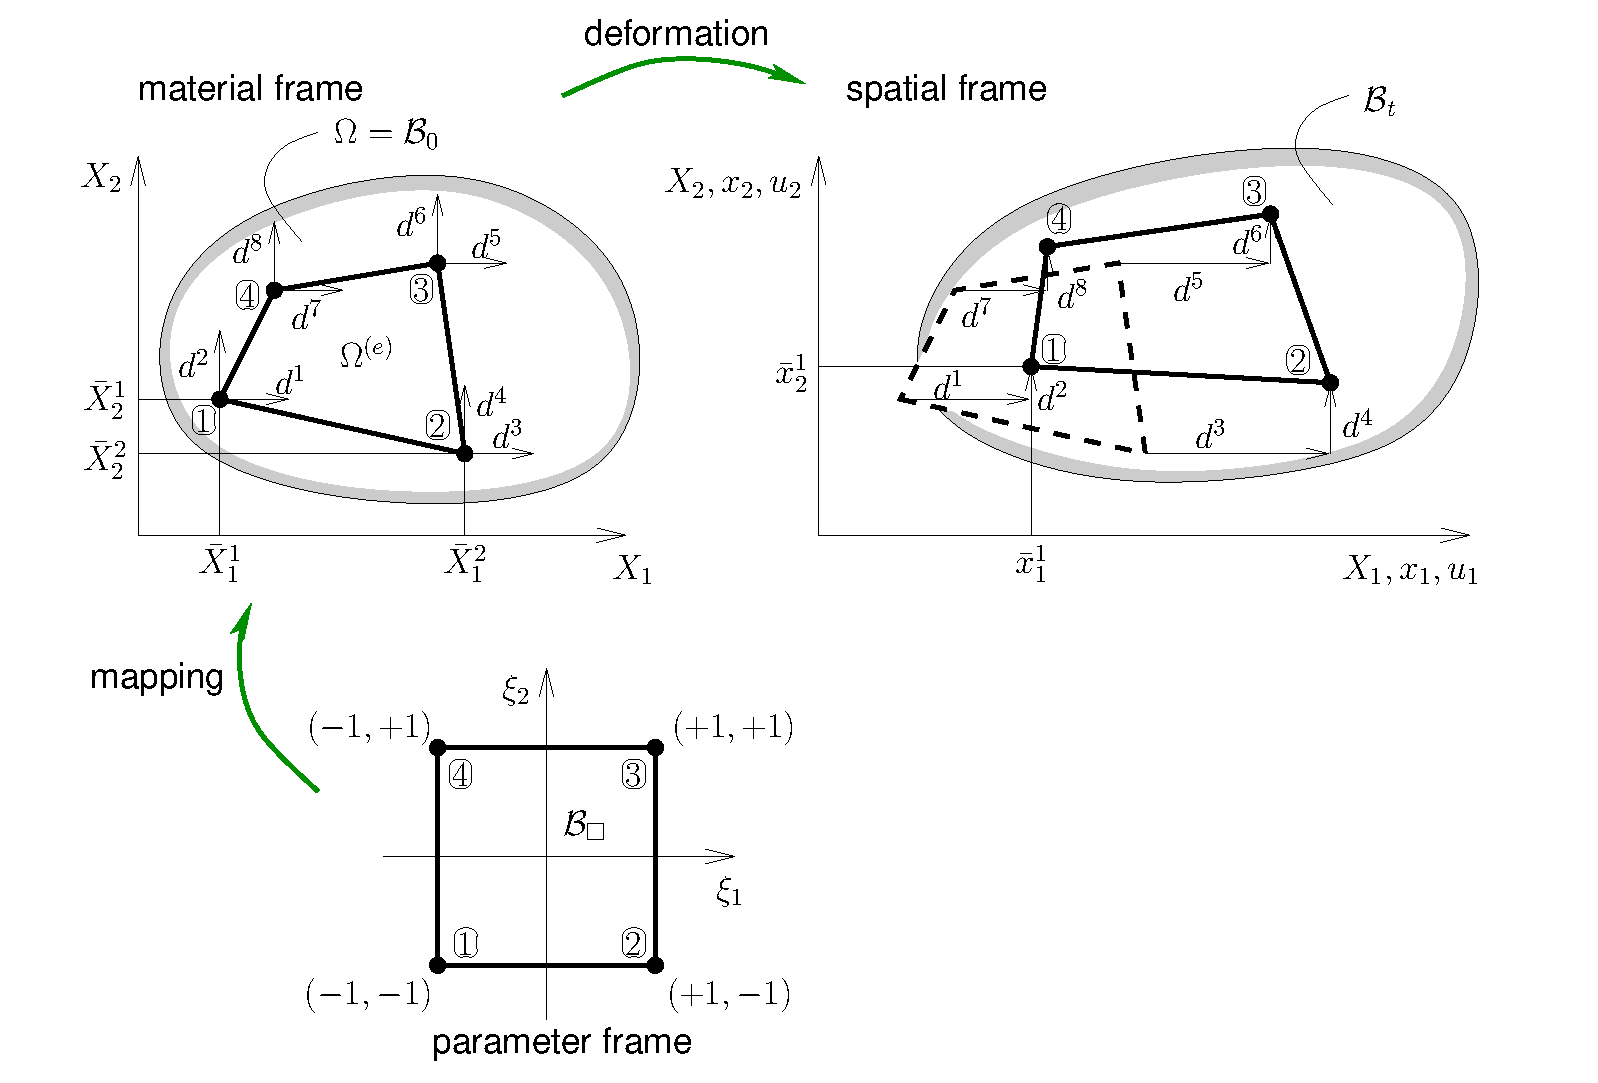
\includegraphics[width=0.8\linewidth]{eps/walleas_element_and_mappings}
\end{center}
\caption{Element geometry of $4$-node EAS wall element}
\label{wall1:fig:eas-wall-element-geometry}
\end{figure}

\subitempart{Jacobian}\\
As usually the Jacobian matrix is established by differentiation
\begin{equation}
  \tns{J}
  = \left[\begin{array}{cc}
    \frac{\pd X_1}{\pd \xi_1}  &  \frac{\pd X_2}{\pd \xi_1}
  \\[1ex]
    \frac{\pd X_1}{\pd \xi_2}  &  \frac{\pd X_2}{\pd \xi_2}
  \end{array}\right]
  = \left[\begin{array}{c}
    \big( \mat{N}_{,\xi_1} \barvct{X} \big)^\T
  \\
    \big( \mat{N}_{,\xi_2} \barvct{X} \big)^\T
  \end{array}\right]
  \qquad\text{and}\qquad
  J
  = \det\tns{J}
  = \frac{\pd X_{1}}{\pd \xi_1} \frac{\pd X_{2}}{\pd \xi_2} -
  \frac{\pd X_{1}}{\pd \xi_2} \frac{\pd X_{2}}{\pd \xi_1} 
  \period
\end{equation}

It allows to map quantities in parameter space to the material
(or undeformed configuration). The inverse
is simply
\begin{equation}
  \tns{J}^{-1} 
  = \frac{1}{\det \tns{J}} \left[ \begin{array}{rr}
    \frac{\pd X_{2}}{\pd \xi_2} & - \frac{\pd X_{2}}{\pd \xi_1} 
  \\[1ex] 
    - \frac{\pd X_{1}}{\pd \xi_2} & \frac{\pd X_{1}}{\pd \xi_1} 
  \end{array} \right]
  \period
\end{equation}
Its inverse $\tns{J}^{-1}$ is of paramount
importance to refer material derivatives to the parameter frame.
\begin{equation}
  \left[\begin{array}{r} 
    \partial_{X_{1}} () 
  \\ 
    \partial_{X_{2}} () 
  \end{array}\right] 
  = \tns{J}^{-1} \left[ \begin{array}{c} 
    \partial_{\xi_1} () 
  \\
    \partial_{\xi_2} () 
  \end{array} \right]
\end{equation}


\subitempart{Jacobian at origin}\\
The Jacobian and its inverse are evaluated at a point
$\vct{\xi}\in\set{B}_\Box$. Eventually, these points are the \name{Gauss}
integration points occurring in the quadrature of the element internal forces,
etc\@. It is convenient to define
\begin{equation}
  \tns{J}_o = \left.\tns{J}\right|_{\vct{\xi}=\vct{0}}
  \comma\quad
  J_o = \det\tns{J}_o
  \quad\text{and inverted}\quad
  \tns{J}_o^{-1} = \left.\tns{J}^{-1}\right|_{\vct{\xi}=\vct{0}}
\end{equation}
i.e.\@ the Jacobian determined at the parametric origin $\vct{\xi}=\vct{0}$. 


%%
%%----------------------------
\subsubsection{Displacement field}

\subitempart{Discretization}\\
The displacement field of a $4$-node quadrilateral wall element engages the
well-known bi-linear Lagrangean shape functions $\mat{N}$ and nodal element
displacements $\vct{d}$:
\begin{equation}
  \vct{u}^{(e)}(\vct{\xi})
  = \mat{N}(\vct{\xi}) \, \vct{d}^{(e)}
  \qquad\text{on $\set{B}_\Box$}
  \period
\end{equation}
The virtual displacements are analogously defined.

\subitempart{Displacement-based deformation gradient}\\
The displacements contribute to the deformation gradient that is given in vector, matrix
and tensor form:
\begin{align}\label{wall1:eq:eas-discrete-displacement-based-deformation-gradient}
  \tilvct{F}^{u(e)}
& = \begin{bmatrix} 
    F_{11}^{u} \\ F_{22}^{u} \\ F_{12}^{u} \\ F_{21}^{u} 
    \end{bmatrix}
%  = \tilvct{1} + \tilvct{H}
  = \tilvct{1} + \mat{B}_\LL \vct{d}
&& \comma
& \barmat{F}^{u(e)}
& = \begin{bmatrix}
    F_{11}^u & 0 & F_{12}^u
  \\
    0 & F_{22}^u & F_{21}^u
  \\
    0 & F_{12}^u & F_{11}^u
  \\
    F_{21}^u & 0 & F_{22}^u
  \end{bmatrix}
&& \text{and}
& \tns{F}^{u(e)}
& = \begin{bmatrix} 
    F_{11}^u & F_{12}^u 
  \\ 
    F_{21}^u & F_{22}^u 
  \end{bmatrix}
  \period
\end{align}
For the sake of completeness, the $\mat{B}_\LL$-operator is given as (\cf{}
Sec.~\ref{wall1:sec:wall})
\begin{equation}
  \mat{B}_\LL
  = \left[\begin{array}{cc:cc:cc:cc}
     N_{,X_1}^1 & 0 & N_{,X_1}^2 & 0 & N_{,X_1}^3 & 0 & N_{,X_1}^4 & 0
  \\
     0 & N_{,X_2}^1 & 0 & N_{,X_2}^2 & 0 & N_{,X_2}^3 & 0 & N_{,X_2}^4
  \\
     N_{,X_2}^1 & 0 & N_{,X_2}^2 & 0 & N_{,X_2}^3 & 0 & N_{,X_2}^4 & 0
  \\
     0 & N_{,X_1}^1 & 0 & N_{,X_1}^2 & 0 & N_{,X_1}^3 & 0 & N_{,X_1}^4
  \end{array}\right]  
\end{equation}

In general, this deformation gradient leads to different values for any point
$\vct{\xi}\in\set{B}_\Box$. We will require the deformation gradient at the
origin ($\vct{\xi}=\vct{0}$) subsequently. We define
\begin{align}
   \tilvct{F}_o^{u(e)}
&  = \left.\tilvct{F}^{u(e)}\right|_{\vct{\xi}=\vct{0}}
&& \comma
&  \barmat{F}_o^{u(e)}
&  = \left.\barmat{F}^{u(e)}\right|_{\vct{\xi}=\vct{0}}
&& \text{and}
&  \tns{F}_o^{u(e)}
&  = \left.\tns{F}^{u(e)}\right|_{\vct{\xi}=\vct{0}}
\end{align}



%%
%%----------------------------
\subsubsection{Enhanced strain field}

\subitempart{Discretization approach}\\
The enhanced strain is disretized by\\
\begin{equation}\label{wall1:eq:eas-enhanced-strain-approach}
\begin{aligned}
  \tns{F}^{\enh(e)}
&  = \sum_{\epsilon=1}^{\eenh=4} \tns{F}_\epsilon^{\enh(e)}
  = \sum_{\epsilon=1}^{\eenh=4} \tns{F}_o^u \cdot \frac{J_o}{J} \tns{J}_o^\T
  \cdot \tns{M}_\epsilon(\vct{\xi}) \alpha_\epsilon \cdot \tns{J}_o^{-\T}
&& \text{on $\set{B}_\Box$}
\end{aligned}
\end{equation}
with the $\eenh=4$ shape functions on $\set{B}_\Box$\\
\begin{equation}\label{wall1:eq:eas-shape-functions-enhanced-strains}
\begin{aligned}
  \tns{M}_1
& = \left[\begin{array}{cc} \xi_1 & 0 \\ 0 & 0 \end{array}\right]
  \comma
& \tns{M}_2
& = \left[\begin{array}{cc} 0 & \xi_2 \\ 0 & 0 \end{array}\right]
  \comma
& \tns{M}_3
& = \left[\begin{array}{cc} 0 & 0 \\ \xi_1 & 0 \end{array}\right]
  \comma
& \tns{M}_4
& = \left[\begin{array}{cc} 0 & 0 \\ 0 & \xi_2 \end{array}\right]
  \period
\end{aligned}
\end{equation}
The parameters $\alpha_\epsilon$ are the \intro{discrete enhanced strain
scalers}. These scalars are determined throughout the computation. They are
ordered in a vector\\
\begin{equation}
  \vct{\alpha}^{(e)}
  = \left[\begin{array}{c}
    \alpha_1 \\ \alpha_2 \\ \alpha_3 \\ \alpha_4
  \end{array}\right]
  \period
\end{equation}


The design of these shape functions respects the following:
\begin{description}
\item[(i) Discontinuity (hybrid):] The shape functions of an element are
  simply considered independent of all surrounding elements. The parameters
  $\vct{\alpha}^{(e)}$ are not shared among different elements.
\item[(ii) Null intersection:] The enhanced gradients
  $\tns{F}^\enh$ are not
  contained in the conforming, displacement-based approximation $\tns{F}^u$,
  i.e.\@ $\tns{F}^\enh$ is an \emph{enrichment} to  $\tns{F}^u$.
\item[(iii) Orthogonality condition:] We demand that
  \begin{equation}
    \int_\Omega \tns{P} : \tns{F}^\enh \, \dd V
    = \sum_{e=1}^{\nele} \int_{\Omega^{(e)}} \tns{P}^{(e)} :
    \tns{F}^{\enh^{(e)}} \, \dd V
    = 0
    \comma
  \end{equation}
  i.e.\@ the enhanced gradient is orthogonal on the 1st
  \name{Piola}--\name{Kirchhoff} stress.

  The incompatible approach of the enhanced strains allows to write element by
  element
  \begin{equation}\label{wall1:eq:eas-orthogonality-condition}
    0 = \int_{\Omega^{(e)}} 
    \tns{P}^{(e)} : \tns{F}^{\enh^{(e)}} \, \dd V
    \qquad\text{for every $e=1,\ldots,\nele$}
    \period
  \end{equation}
  Moreover, due to the incompatible approach, the virtual counterparts
  $\virt\tns{P}^{(e)}$ and $\virt\tns{F}^{\enh(e)}$ belong to the same function
  space as $\tns{P}^{(e)}$ and $\tns{F}^{\enh(e)}$, respectively. Thus, the
  following equations vanish as well
  \begin{align}
     0 & = \int_{\Omega^{(e)}} 
     \virt\tns{P}^{(e)} : \tns{F}^{\enh^{(e)}} \, \dd V
     && \text{and}
     & 0 & = \int_{\Omega^{(e)}} 
     \tns{P}^{(e)} : \virt\tns{F}^{\enh^{(e)}} \, \dd V
  \end{align}
  Consequently, these two terms vanish in the weak form,
  Eq.~\eqref{wall1:eq:eas-weak-form-StVenantKirchhoff}.

  Introducing the shape functions Eq.~\eqref{wall1:eq:eas-enhanced-strain-approach},
  we obtain 
  \begin{equation}
  \begin{split}
    0 
  & = \int_{\Omega^{(e)}}
      \tns{P}^{(e)\T} : \tns{F}^{\enh(e)} \, \dd V
  \\
  & = \int_{\Omega^{(e)}}
       \tns{P}^{(e)\T} : \Big(\sum_{\epsilon=1}^{\eenh} 
      \tns{F}_o^u \cdot \frac{J_o}{J} \tns{J}_o^\T \cdot \tns{M}_\epsilon(\vct{\xi})
    \alpha_\epsilon \cdot \tns{J}_o^{-\T} \Big) \, \dd V
  \end{split}
  \end{equation}
  We want that $\mat{P}^{(e)}$ can take on at least constant stresses. In
  this case the condition arises:
  \begin{equation}
  \begin{split}
    \vct{0} 
  & = \int_{\Omega^{(e)}} \Big(
      \sum_{\epsilon=1}^{\eenh} 
      \tns{F}_o^u \cdot \frac{J_o}{J} \tns{J}_o^\T \cdot
  \tns{M}_\epsilon(\vct{\xi}) 
    \alpha_\epsilon \cdot \tns{J}_o^{-\T} \Big)
    \, \dd V
  \\
  & = \tns{F}_o^u \cdot J_o \tns{J}_o^\T \cdot T \Big\{
    \sum_{\epsilon=1}^{\eenh} \Big( \int_{\set{B}_\Box}
    \tns{M}_\epsilon(\vct{\xi}) \, \dd\vct{\xi} \, \alpha_\epsilon \Big) \Big\}
    \cdot \tns{J}_o^{-\T}
  \end{split}
  \end{equation}
  The thickness of the wall element is denoted $T$. 
  Generally, this condition can only be satisfied if the integral 
  \begin{equation}
    \mat{0}
    = \int_{\set{B}_\Box} \tns{M}_\epsilon(\vct{\xi}) \, \dd\vct{\xi}
    = \int_{\xi_1=-1}^{+1}\int_{\xi_2=-1}^{+1} \tns{M}_\epsilon(\vct{\xi}) \,
    \dd\vct{\xi}
    \qquad\text{for every $\epsilon=1,\ldots,\eenh$}
    \period
  \end{equation}
  The symmetric integration bounds permit to say that every odd function
  satisfies the condition. Every odd polynomial in $\xi_1$ and $\xi_2$ is an
  odd function, for instance $\int_{-1}^{+1}\int_{-1}^{+1} \xi_1
  \,\dd\vct{\xi} = 2 \, \big[ \frac{1}{2} \xi_1^2 \big]_{-1}^{+1} = 0$. This
  is exactly the case for all shape functions in 
  \eqref{wall1:eq:eas-shape-functions-enhanced-strains}.
\item[(iv) Frame invariance (objectivity):] The presence of $\mat{F}_o^u$
  in \eqref{wall1:eq:eas-enhanced-strain-approach} assures that the final
  deformation gradient (and thus the final finite 
  element formulation) exhibits the proper invariance properties under change
  of observer, leading to an objective (frame-indifferent) formulation.
\end{description}

\subitempart{Matrix and vector notation}\\
The enhanced strain tensor \eqref{wall1:eq:eas-enhanced-strain-approach} can be
denoted in a vector, \ie{}
\begin{equation}\label{wall1:eq:eas-enhanced-strain-vectorially}
  \tilvct{F}^{\enh(e)}
  = \begin{bmatrix} 
    F_{11}^\enh \\ F_{22}^\enh \\ F_{12}^\enh \\ F_{21}^\enh 
  \end{bmatrix}
  = \underbrace{\begin{bmatrix}
    G_{11;1} & G_{11;2} & G_{11;3} & G_{11;4}
  \\
    G_{22;1} & G_{22;2} & G_{22;3} & G_{22;4}
  \\
    G_{12;1} & G_{12;2} & G_{12;3} & G_{12;4}
  \\
    G_{21;1} & G_{21;2} & G_{21;3} & G_{21;4}
  \end{bmatrix}}_{\mat{G}}
  \underbrace{\begin{bmatrix}
    \alpha_1 \\ \alpha_2 \\ \alpha_3 \\ \alpha_4
  \end{bmatrix}}_{\vct{\alpha}}
\end{equation}
in which a column vector $\tilvct{G}_\epsilon$ of $\mat{G}$ is the vectorial
form of (\cf{} Eq.~\eqref{wall1:eq:eas-enhanced-strain-approach})
\begin{align}
  \tns{F}_\epsilon^{\enh(e)}
& = \underbrace{\tns{F}_o^u \cdot \frac{J_o}{J} \tns{J}_o^\T
  \cdot \tns{M}_\epsilon(\vct{\xi}) \cdot \tns{J}_o^{-\T}}
  _{\displaystyle\tns{G}_\epsilon}
  \; \alpha_\epsilon
&&\Longrightarrow
& \tilvct{G}_\epsilon
& = \begin{bmatrix}
    G_{11;\epsilon} \\ G_{22;\epsilon} \\ G_{12;\epsilon} \\ G_{21;\epsilon}
  \end{bmatrix}
\end{align}

Due to the linear dependence of the enhanced gradient
$\tilvct{F}^\enh$ on the scalers $\vct{\alpha}$, the derivative of
$\tilvct{F}^\enh$ with respect to $\vct{\alpha}$ is simply $\mat{G}$. Please
note, the $\mat{G}$-operator depends on the discrete element displacements,
because $\tns{F}_o^u$ does.

The matrix $\barmat{F}^{\enh(e)}$ is specified similarly to
\eqref{wall1:eq:eas-discrete-displacement-based-deformation-gradient}. 

%%
%%----------------------------
\subsubsection{\name{St.~Venant}--\name{Kirchhoff} constitutive relation}
The discretized total deformation gradient is
\begin{align}
  \tilvct{F}
& = \tilvct{F}^u
  + \tilvct{F}^\enh
&&\text{and}
& \barmat{F}
& = \barmat{F}^u
  + \barmat{F}^\enh
  \period
\end{align}
The \name{Green}--\name{Lagrange} strain accumulates in
\begin{equation}
  \vct{E}^F
  = \tfrac{1}{2} \big( \barmat{F}^\T \tilvct{F} - \vct{1} \big)
\end{equation}
The discrete 1st \name{Piola}--\name{Kirchhoff} stress vector in the context
of \name{St.~Venant}--\name{Kirchhoff} material results in
\begin{equation}\label{wall1:eq:eas-1st-pk-stress}
  \tilvct{P}^F
  = \begin{bmatrix}
    P_{11} \\ P_{22} \\ P_{12} \\ P_{21}
  \end{bmatrix}^F
  = \barmat{F}
    \, \underbrace{\mat{C}_\VK \, \vct{E}^F}_{\displaystyle\vct{S}^F}
\end{equation}

\subsubsection{Internal element force vector and linearization}
\label{wall1:sec:eas-intforce-linearisation}
\subitempart{Element-wise enhanced strain three-field variational form}\\
Let us return to the principle of virtual work \eqref{wall1:eq:eas-virtwork}
integrated on element domains $\Omega^{(e)}$ with cancelled terms due to the
orthogonality condition
\begin{equation}
  \sum_{e=1}^{\nele} \Bigg[
    \int_{\Omega^{(e)}}  \underbrace{\virt\tns{F}^u}_{\Grad\virt\tns{u}}
    : \tns{P}^F\, \dd V
    + \int_{\Omega^{(e)}} \virt\tns{F}^\enh : \tns{P}^F \, \dd V
    - \virt W_\Ext^{(e)}
  \Bigg]
  = 0
\end{equation}
This can be denoted in matrix fashion
\begin{equation}
  \sum_{e=1}^{\nele} \Bigg[
    \int_{\Omega^{(e)}} \virt\tilvct{F}^{u\T} \tilvct{P}^{F}  \, \dd V
    + \int_{\Omega^{(e)}} \virt\tilvct{F}^{\enh\T} \tilvct{P}^{F}  \, \dd V
    - \virt W_\Ext^{(e)}
  \Bigg]
  = 0
  \period
\end{equation}
The discretized virtual deformation gradients are referred back to the virtual
nodal displacements and enhanced strain scalers:
\begin{equation}\label{wall1:eq:eas-virt-work-in-virt-displ}
  \sum_{e=1}^{\nele} \Bigg[
    \underbrace{\int_{\Omega^{(e)}} 
      \big(\tilvct{F}_{,\vct{d}}^{u} \, \virt\vct{d} 
           + \tilvct{F}_{,\vct{d}}^{\enh} \,\virt\vct{d} \big)^\T
      \tilvct{P}^{F}  \, \dd V}_{\displaystyle \leadsto \;\; \virt\vct{d}^\T\vct{f}_\Int^{(e)}}
    + \underbrace{\int_{\Omega^{(e)}} 
      \big(\tilvct{F}_{,\vct{\alpha}}^{\enh} \,\virt\vct{\alpha} \big)^\T 
      \tilvct{P}^{F}  \, \dd V}_{\displaystyle\leadsto \;\; \virt\vct{\alpha}^\T\vct{s}^{(e)}}
    - \virt\vct{d}^\T \vct{f}_\Ext^{(e)}
  \Bigg]
  = 0
  \comma
\end{equation}
here the left integral contains the variations of both discretized deformation
gradients with respect to $\vct{d}$. The enhanced gradient
depends on $\vct{\alpha}$ and $\vct{d}$ as well. The dependence on the virtual
displacements stems from the deformation gradient $\tns{F}_o^u$ occurring in
\eqref{wall1:eq:eas-enhanced-strain-approach}. 

\subitempart{Element load vector}\\
The external virtual work leads to
the external element load vector
\begin{equation}
  \vct{f}_\Ext^{(e)} 
  = \int_{\Omega^{(e)}} \mat{N}^\T \hatvct{b}_0 \, \dd V
  + \int_{\Gamma_\sig^{(e)}} \mat{N}^\T \hatvct{t}_0 \, \dd A
\end{equation}
as shown in Sec.~\ref{wall1:sec:wall}.

\subitempart{Internal element force vector}\\
Looking at \eqref{wall1:eq:eas-virt-work-in-virt-displ} we need
$\tilvct{F}_{,\vct{d}}^u$ and $\tilvct{F}_{,\vct{d}}^\enh$ to define the
internal force vector
\begin{equation}
  \vct{f}_\Int^{(e)}
  = \int_{\Omega^{(e)}} \big(\tilvct{F}_{,\vct{d}}^{u}
           + \tilvct{F}_{,\vct{d}}^{\enh} \big)^\T
      \tilvct{P}^{F}  \, \dd V
  \period
\end{equation}
Straightforwardly we achieve 
\begin{equation}
  \tilvct{F}_{,\vct{d}}^u = \mat{B}_\LL
\end{equation}
%$\tilvct{F}_{,\vct{\alpha}}^\enh = \mat{G}$. 
The missing $\tilvct{F}_{,\vct{d}}^\enh$ is obtained by rewriting
\eqref{wall1:eq:eas-enhanced-strain-approach} 
\begin{align}
  \tns{F}^{\enh(e)}
& = \tns{F}_o^u \cdot \underbrace{
  \frac{J_o}{J} \tns{J}_o^\T
  \cdot \sum_{\epsilon=1}^{\eenh} \Big( 
    \tns{M}_\epsilon \, \alpha_\epsilon 
  \Big) \cdot \tns{J}_o^{-\T}}
  _{\displaystyle\tns{A}(\vct{\alpha})}
&&\text{with}
& \tns{A}
& = \begin{bmatrix}
  A_{11} & A_{12} \\ A_{21} & A_{22}
  \end{bmatrix}
\end{align}
A reshaping of $\tns{A}$ in the matrix $\barmat{A}$ allows to define concisely
\begin{equation}
  \tilvct{F}^{\enh(e)}
  = \underbrace{\begin{bmatrix} 
    A_{11} & 0 & A_{21} & 0
  \\
    0 & A_{22} & 0 & A_{12}
  \\
    A_{12} & 0 & A_{22} & 0
  \\
    0 & A_{21} & 0 & A_{11}
  \end{bmatrix}}_{\displaystyle\barmat{A}}
  \; \underbrace{\begin{bmatrix}
    F_{11}^u \\ F_{22}^u \\ F_{12}^u \\ F_{21}^u
  \end{bmatrix}_o}_{\displaystyle\tilvct{F}_o^u}
\end{equation}
The matrix $\barmat{A}$ does not depend on the nodal displacements, however,
it contains the enhanced gradient scalers. 
The differentiation of $\tilvct{F}^{\enh(e)}$ with respect to $\vct{d}$
is readily 
\begin{equation}\label{wall1:eq:eas-enhanced-strain-differentiated-displacements}
  \tilvct{F}_{,\vct{d}}^{\enh(e)} \, \virt\vct{d}
  = \barmat{A} \, \virt\tilvct{F}_{o,\vct{d}}^{u(e)}
  = \barmat{A} \, \underneath{\mat{B}_{\LL o}}{\mat{B}_{\LL o}=\left.\mat{B}_\LL\right|_{\vct{\xi}=\vct{0}}} \, \virt\vct{d}
  = \mat{W}_o \, \virt\vct{d}
\end{equation}

\subitempart{Enhancement equation vector}\\
The \intro{enhancement equation vector} $\vct{s}^{(e)}$ is due to
\eqref{wall1:eq:eas-virt-work-in-virt-displ}:
\begin{equation}\label{wall1:eq:eas-constraint-vector}
  \vct{s}^{(e)}
  = \int_{\Omega^{(e)}} \tilvct{F}_{,\vct{\alpha}}^{\enh\,\T} \tilvct{P}^{F}
  \, \dd V
\end{equation}
Easily, the derivative of $\tilvct{F}^{\enh}$ with respect to $\vct{\alpha}$
is identified with \eqref{wall1:eq:eas-enhanced-strain-vectorially}
\begin{equation}
    \tilvct{F}_{,\vct{\alpha}}^{\enh}
  = \mat{G}
  \period
\end{equation}


$\Longrightarrow$ The sum of discretized virtual work of each element is
hence\\
\begin{equation}
  \sum_{e=1}^{\nele} \Bigg[
  \underbrace{\virt\vct{d}^\T \int_{\Omega^{(e)}} 
    \big(\mat{B}_\LL + \mat{W}_o \big)^\T \tilvct{P}^F
  \,\dd V}_{\boxed{1}}
  \;+\; \underbrace{\virt\vct{\alpha}^\T \int_{\Omega^{(e)}} 
    \mat{G}^\T \tilvct{P}^F
  \,\dd V}_{\boxed{2}}
  \;-\; \underbrace{\virt\vct{d}^\T \vct{f}_\Ext^{(e)}}_{\boxed{3}}
  \Bigg]
  = 0
\end{equation}
in which the virtual quantities are factored out of the integrals as they are
here discrete quantities.

\subitempart{Assembly}\\
The virtual element displacements $\virt\vct{d}$ are part of the
\emph{continuous} displacement approach across element boundaries. We need to
assemble the terms $\boxed{1}$ and $\boxed{3}$. The virtual  scalers
$\virt\vct{\alpha}$ belong to the \emph{discontinuous} enhanced 
gradient discretization. Thus term $\boxed{2}$ must be zero
separately  on each element.

\begin{equation}
\left\{\begin{split}
  0
& =
  \virt\vct{D}^\T \Ass{e=1}{\nele} \Bigg[
    \overbrace{\displaystyle\int_{\Omega^{(e)}} 
      \big(\mat{B}_\LL + \mat{W}_o \big)^\T \tilvct{P}^F
    \,\dd V}^{\vct{f}_\Int^{(e)}(\vct{d},\vct{\alpha})}
    \;-\; \vct{f}_\Ext^{(e)}
  \Bigg]
\\
  0
& =
  \virt\vct{\alpha}^\T \underbrace{\int_{\Omega^{(e)}} 
    \mat{G}^\T \tilvct{P}^F
  \,\dd V}_{\displaystyle\vct{s}^{(e)}(\vct{d},\vct{\alpha})}
  \qquad\text{for every $e=1,\ldots,\nele$}
\end{split}\right.
\end{equation}
These equations must vanish for any permissible virtual displacement and
strain scaling, with $\mat{\Alpha} =
\begin{bmatrix}\vct{\alpha}^{(1)}&\cdots&\vct{\alpha}^{(\nele)}\end{bmatrix}$, 
\begin{equation}
\left\{\begin{split}
  \vct{0}
& = \Ass{e=1}{\nele} \Big[
  \vct{f}_\Int(\vct{d},\mat{\alpha})
  \;-\; \vct{f}_\Ext
  \Big]^{(e)}
  \qquad\Longrightarrow\qquad
  \vct{0}
  = \vct{F}_\Int(\vct{D},\mat{\Alpha})
  - \vct{F}_\Ext
  = \vct{R}(\vct{D},\mat{\Alpha})
\\
  \vct{0}
& = \vct{s}^{(e)}(\vct{d},\vct{\alpha})
  \qquad\text{for every $e=1,\ldots,\nele$}
\end{split}\right.  
\end{equation}
The equilibrium equations are an $\ndof$-dimensional global system of
equations coupled to the $\nele\times\eenh$ element-wise equation
systems. These systems together permit the determination of $\vct{D}$
($\ndof$-dimensional vector) and $\mat{\Alpha} =
\begin{bmatrix}\vct{\alpha}^{(1)}&\cdots&\vct{\alpha}^{(\nele)}\end{bmatrix}$
(in total $\nele\times\eenh$ unknowns).

\subitempart{Linearization}\\
The system of equations is nonlinear and a \name{Newton}--\name{Raphson}
iteration can be used to solve it. This solution technique requires the
linearization of the residuals. The linearization is carried out at the
current iterative step $i$:
\begin{equation}\label{wall1:eq:eas-linearisation}
\left\{\begin{split}
& \Lin\vct{R}
  = \vct{R}(\vct{D}^i,\mat{\Alpha}^i)
  + \Ass{e=1}{\nele} \Big[
    \vct{f}_{\Int,\vct{d}}(\vct{d}^i,\mat{\alpha}^i)
    \, \incr\vct{d}^{i+1}
    + \vct{f}_{\Int,\vct{\alpha}}(\vct{d}^i,\mat{\alpha}^i)
    \, \incr\vct{\alpha}^{i+1}
  \Big]^{(e)}
  = \vct{0}
\\
& \Lin\vct{s}^{(e)}
  = \Big[ \, 
    \vct{s}(\vct{d}^i,\vct{\alpha}^i)
  \, \Big]^{(e)}
  + \Big[
    \vct{s}_{,\vct{d}}(\vct{d}^i,\vct{\alpha}^i) \, \incr\vct{d}^{i+1}
    + \vct{s}_{,\vct{\alpha}}(\vct{d}^i,\vct{\alpha}^i)
      \, \incr\vct{\alpha}^{i+1} 
  \Big]^{(e)}
  = \vct{0}
\end{split}\right.
\end{equation}

\subitempart{Stiffness matrices}\\
The differentiated internal force vector and enhanced equation lead to
`stiffness matrices' (tangent matrices). We designate for each element $(e)$
\begin{align}
&
\begin{array}{rl}
  \mat{k}_{dd}^{i(e)}
  = \vct{f}_{\Int,\vct{d}}^{(e)}(\vct{d}^i,\mat{\alpha}^i)
& = \displaystyle\int_{\Omega^{(e)}}
    \big( \mat{B}_\LL + \mat{W}_o \big)^\T 
    \barmat{F} \, \mat{C}_\VK \, \barmat{F}^\T
    \big( \mat{B}_\LL + \mat{W}_o \big)
    \, \dd V
\\[2ex]
& + \displaystyle\int_{\Omega^{(e)}}
    \big( \mat{B}_\LL + \mat{W}_o \big)^\T
    \, \barmat{S}^F \,
    \big( \mat{B}_\LL + \mat{W}_o \big)
    \, \dd V
\end{array}
\\
&
\begin{array}{rl}
  \mat{k}_{d\alpha}^{i(e)}
  = \vct{f}_{\Int,\vct{\alpha}}^{(e)}(\vct{d}^i,\mat{\alpha}^i)
& = \displaystyle\int_{\Omega^{(e)}}
    \big( \mat{B}_\LL + \mat{W}_o \big)^\T 
    \barmat{F} \, \mat{C}_\VK \, \barmat{F}^\T
    \mat{G}
    \, \dd V
\\[2ex]
& + \displaystyle\int_{\Omega^{(e)}}
    \big( \mat{B}_\LL + \mat{W}_o \big)^\T
    \, \barmat{S}^F \,
    \mat{G}
    \, \dd V
\\[2ex]
& + \displaystyle\int_{\Omega^{(e)}}
    \bar{\barmat{P}}^F \mat{Z}
    \, \dd V
\end{array}
\\
&
\begin{array}{rl}
  \mat{k}_{\alpha d}^{i(e)}
  = \vct{s}_{,\vct{d}}^{(e)}(\vct{d}^i,\vct{\alpha}^i)
&  = \big[ \mat{k}_{d\alpha}^{i(e)} \big]^\T
\end{array}
\\
&
\begin{array}{rl}
  \mat{k}_{\alpha\alpha}^{i(e)}
  = \vct{s}_{,\vct{\alpha}}^{(e)}(\vct{d}^i,\vct{\alpha}^i)
& = \displaystyle\int_{\Omega^{(e)}}
    \mat{G}^\T
    \barmat{F} \, \mat{C}_\VK \, \barmat{F}^\T
    \mat{G}
    \, \dd V
\\[2ex]
& + \displaystyle\int_{\Omega^{(e)}}
    \mat{G}^\T
    \, \barmat{S}^F \,
    \mat{G}
    \, \dd V
\end{array}
\end{align}
The following matrices are constructed (with \eqref{wall1:eq:eas-1st-pk-stress} and
\eqref{wall1:eq:eas-enhanced-strain-differentiated-displacements}) by taking into
account redundancies in $\mat{W}_o$
\begin{align}
  \bar{\barmat{P}}^F
& = \left[\begin{array}{cc:cc:cc:cc}
     P_{11} & P_{12} & & & & & &
  \\ P_{21} & P_{22} & & & & & &
  \\ \hdashline
     & & P_{11} & P_{12} & & & &
  \\ & & P_{21} & P_{22} & & & &
  \\ \hdashline
     & & & & P_{11} & P_{12} & &
  \\ & & & & P_{21} & P_{22} & &
  \\ \hdashline
     & & & & & & P_{11} & P_{12}
  \\ & & & & & & P_{21} & P_{22}
  \end{array}\right]
&&\text{and}
& \tilde{\tilvct{Z}}_\epsilon
& = \left[\begin{array}{cccc}
     W_{o11,\alpha_\epsilon}
  \\ W_{o22,\alpha_\epsilon}
  \\ \hdashline 
     W_{o13,\alpha_\epsilon}
  \\ W_{o24,\alpha_\epsilon}
  \\ \hdashline 
     W_{o15,\alpha_\epsilon}
  \\ W_{o26,\alpha_\epsilon}
  \\ \hdashline 
     W_{o17,\alpha_\epsilon}
  \\ W_{o28,\alpha_\epsilon}
  \end{array}\right]
\end{align}
(with, for instance, $W_{o11,\alpha_\epsilon} = \frac{\pd W_{o11}}{\pd
  \alpha_\epsilon}$) and
\begin{equation}
  \mat{Z}
  = \begin{bmatrix}
    \tilde{\tilvct{Z}}_1 & \cdots & \tilde{\tilvct{Z}}_\eenh
  \end{bmatrix}
  \period
\end{equation}

The linearized discrete equations, \eqref{wall1:eq:eas-linearisation}, are now
written
\begin{equation}\label{wall1:eq:eas-linearisation-with-stiffness}
\left\{\begin{split}
  \vct{0}
& = \Ass{e=1}{\nele} \Big[
    \vct{f}_\Int^{i} - \vct{f}_\Ext
    \Big]^{(e)}
  + \Ass{e=1}{\nele} \Big[
    \mat{k}_{dd}^i \incr\vct{d}^{i+1}
    + \mat{k}_{d\alpha}^i \incr\vct{\alpha}^{i+1}
    \Big]^{(e)}
\\
  \vct{0}
& = \vct{s}^i
  + \Big[ \mat{k}_{\alpha d}^i \incr\vct{d}^{i+1}
    + \mat{k}_{\alpha\alpha}^i \incr\vct{\alpha}^{i+1}
    \Big]
  \qquad\text{for each $e=1,\ldots,\nele$}
\end{split}\right.
\end{equation}
The left assembly results in $\vct{R}(\vct{D}^i,\mat{\Alpha}^i)$. 

\subitempart{Statically condensed internal force and stiffness}\\
The second equation for $\vct{s}^{i(e)}$ in \eqref{wall1:eq:eas-linearisation-with-stiffness} holds
for individual elements (owing to the discontinuous approach of the strain
enhancement). Therefore, the equation can be solved at the element level for
$\incr\vct{\alpha}^{i+1}$:\\
\begin{equation}\label{wall1:eq:eas-enhanced-strain-increments}
  \incr\vct{\alpha}^{i+1}
  = - \big[ \mat{k}_{\alpha\alpha}^i \big]^{-1}
  \big( \vct{s}^{i} + \mat{k}_{\alpha d}^i \, \incr\vct{d}^{i+1} \big)
  \period
\end{equation}
Equation \eqref{wall1:eq:eas-enhanced-strain-increments} is sent to the first
equation in \eqref{wall1:eq:eas-linearisation-with-stiffness} resulting in the
statically condensed (or reduced, \ger{statisch kondensiert}) form\\
\begin{equation}[2cm]
  \vct{0}
  = \underbrace{\Ass{e=1}{\nele} \Big[
    \underbrace{\vct{f}_\Int^i 
    - \mat{k}_{d\alpha}^i \big[\mat{k}_{\alpha\alpha}^{i}\big]^{-1} \vct{s}^i}
    _{\displaystyle\vct{f}_{\Int\,\red}^{i(e)}}
    - \vct{f}_\Ext
    \Big]^{(e)}}_{\displaystyle\vct{F}_{\Int\,\red}(\vct{D}^i,\mat{\Alpha}^i)-\vct{F}_\Ext}
  + \underbrace{\Ass{e=1}{\nele} \Big[
    \underbrace{\big(\mat{k}_{dd}^i 
    - \mat{k}_{d\alpha}^i \big[\mat{k}_{\alpha\alpha}^{i}\big]^{-1}
    \mat{k}_{\alpha d}^i \big)}_{\displaystyle\mat{k}_\red^{i(e)}}
    \incr\vct{d}^{i+1} 
    \Big]^{(e)}}_{\displaystyle\mat{K}_{\Tang\red}^i \, \incr\vct{D}^{i+1}}
\end{equation}
After assembling we achieve the usual \name{Newton}--\name{Raphson} iterative
increments formula
\begin{equation}
  \incr\vct{D}^{i+1}
  = -\big[ \mat{K}_{\Tang\red}^i \big]^{-1} \, \vct{R}^i
  = -\big[ \mat{K}_{\Tang\red}^i \big]^{-1}
    \big( \vct{F}_{\Int\,\red}(\vct{D}^i,\mat{\Alpha}^i)-\vct{F}_\Ext \big)
\end{equation}

\subitempart{Load-controlled algorithm}\\
The complete load-controlled algorithm utilizes the
\name{Newton}--\name{Raphson} iteration (NRI) in such a way,
Fig.~\ref{wall1:fig:eas-load-controlled-algo}.

\begin{figure}[H]
\begin{center}
\begin{struktogramm}(145,125)
\assign{Read initial load factor / conditions: $\lambda_0=0$, $\vct{D}_0=\vct{0}$\\
  Get enhanced strain scalers: $\mat{\Alpha}_0=\mat{0}$}
\while{Loop over load steps $k=0,1,\ldots$ while $\lambda_k\leq\lambda_{max}$}
   \assign{Predictor (constant): 
     $\vct{D}_{k+1}^{i=0}:=\vct{D}_{k}$ 
     and $\mat{\Alpha}_{k+1}^{i=0}:=\mat{\Alpha}_k$}
   \assign{Load vector: $\vct{F}_{\Ext}(\lambda_{k+1})$}
   \assign{Residual: $\vct{R}(\vct{D}_{k+1}^{i=0},\mat{\Alpha}_{k+1}^{i=0})
     = \vct{F}_{\Int\,\red}(\vct{D}_{k+1}^{i=0},\mat{\Alpha}_{k+1}^{i=0})
     - \vct{F}_{\Ext}(\lambda_{k+1})$}
   \while{Newton loop $i=0,1,\ldots$  while $\Abs{
       \vct{R}(\vct{D}_{k+1}^{i},\mat{\Alpha}_{k+1}^i) } > \tol$}
      \assign{Assemble red.\@ stiffness matrix:
        $\mat{K}_{\Tang\red}^i$}
      \assign{Solve displ. iter. incr.: 
        $\Delta\vct{D}_{k+1}^{i+1} 
        = -\big[\mat{K}_{\Tang\,\red}^i\big]^{-1} \, 
        \vct{R}(\vct{D}_{k+1}^{i},\mat{\Alpha}_{k+1}^i)$}
      \while{Element loop $e=1,\ldots,\nele$}
        \assign{Enh.\@ strain scalers iterative increment:\\
          $\incr\vct{\alpha}_{k+1}^{i+1(e)}
          = - \big[ \mat{k}_{\alpha\alpha}^{i(e)} \big]^{-1}
          \big( \vct{s}_{k+1}^{i(e)} 
          + \mat{k}_{\alpha d}^{i(e)} \, \incr\vct{d}_{k+1}^{i+1(e)} \big)$}
        \assign{Update enh.\@ strain scalers:
          $\vct{\alpha}_{k+1}^{i+1(e)} 
          := \vct{\alpha}_{k+1}^{i(e)} + \incr\vct{\alpha}_{k+1}^{i+1(e)}$\\
          $\Longrightarrow$ 
          $\mat{\Alpha}_{k+1}^{i+1}
          := \begin{bmatrix} \cdots & \vct{\alpha}_{k+1}^{i+1(e)} 
          & \cdots \end{bmatrix}$}
      \whileend
      \assign{Update displacements: 
        $\vct{D}_{k+1}^{i+1} := \vct{D}_{k+1}^i + \Delta\vct{D}_{k+1}^{i+1}$}
      \assign{Generate residual:\\
        $\vct{R}(\vct{D}_{k+1}^{i+1},\mat{\Alpha}_{k+1}^{i+1})
        = \vct{F}_{\Int\,\red}(\vct{D}_{k+1}^{i+1},\mat{\Alpha}_{k+1}^{i+1})
        - \vct{F}_{\Ext}(\lambda_{k+1})$}
     \assign{Update iteration counter: $i := i + 1$}
   \whileend
   \assign{Update load step: $k := k+1$}
   \assign{Update load factor: $\lambda_{k+1} := \lambda_k + \incr\lambda$}
\whileend
\end{struktogramm}
\end{center}
\caption{Load-control with NRI using EAS elements}
\label{wall1:fig:eas-load-controlled-algo}
\end{figure}

\subpart{Remark} For the sake of simplicity, we start with $\vct{D}_0=\vct{0}$
and $\lambda_0=0$ at a strain-free state. Hence, the enhancement parameters
are $\mat{\Alpha}_0=\mat{0}$. Of course, we could also start with
an initial displacement $\vct{D}_0\neq\vct{0}$. In this case, the
corresponding enhancement parameters $\mat{\Alpha}_0$ have to be iteratively
identified. 

%%
%%----------------------------
\subsubsection{External element load vector}
The element load vector is identical to the vector of the purely
displacement-based element described in Sec.~\ref{wall1:sec:wall-extforce}.


%%
%%============================
\subsection{Examples}

\subitempart{Cantilever beam}\\
The investigated beam is depicted in
Fig.~\ref{wall1:fig:eas-cantilever-system}\@. The beam is
characterized by $E=4\EE{6}$, $\nu=0$, $L=10$, $h=0.1$ ($\to$ slenderness
$L/h=100$). The beam is subjected
to a load $P=3$ at the free tip.
\begin{figure}[H]
  \begin{center}
    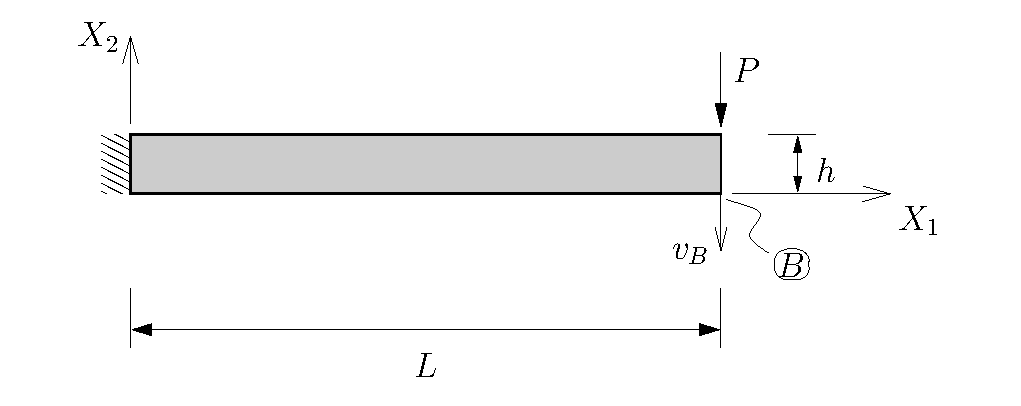
\includegraphics[width=0.6\linewidth]{eps/cant100-beam-system}
  \end{center}
  \caption{Cantilever system}
  \label{wall1:fig:eas-cantilever-system}
\end{figure}
The beam is disretized with $4$-node wall elements
based on plain displacement (Q1) and EAS approaches (Q1E4). Different meshes
are applied: $10\times1$ ($40$), $20\times1$ ($80$), $40\times1$ ($160$),
$100\times1$ ($400$), $200\times2$ ($1200$), $400\times4$ ($4000$) and
$800\times8$ ($14400$) in which the first number indicates the number of
elements in axial direction, the second number in lateral direction and the
number in parentheses the total displacement DOFs. The overall deflection is
displayed in Figure~\ref{wall1:fig:eas-cantilever-deformation} obtained with a
coarse mesh. 
\begin{figure}[H]
  \begin{center}
    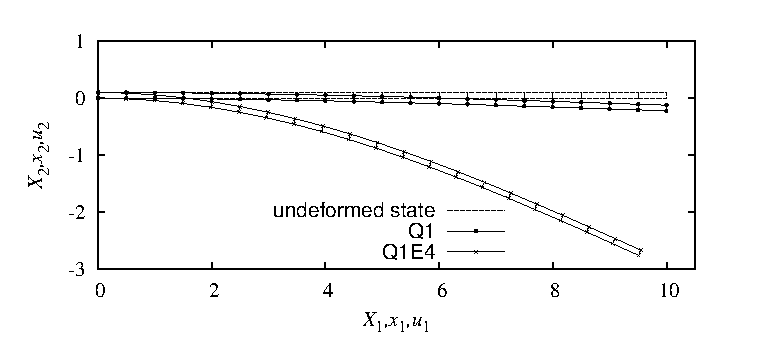
\includegraphics[width=0.9\linewidth]{eps/cant100-system-deformation}
  \end{center}
  \caption{Cantilever example deflection}
  \label{wall1:fig:eas-cantilever-deformation}
\end{figure}
In Fig.~\ref{wall1:fig:eas-convergence-tip-displ-cantilever} the
resulting tip deflection is drawn with respect to the meshes. 
\begin{figure}[H]
  \begin{center}
    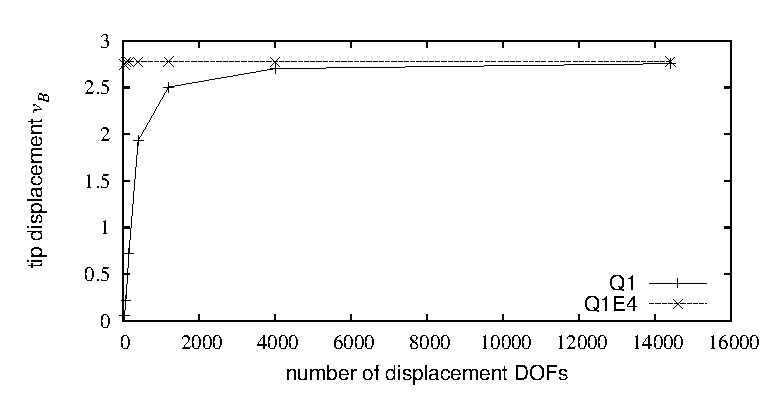
\includegraphics[width=0.8\linewidth]{eps/cant100-tipdispl}
  \end{center}
  \caption{Convergence diagram for tip displacement}
  \label{wall1:fig:eas-convergence-tip-displ-cantilever}
\end{figure}
It can be clearly observed the Q1 elements require a very fine mesh to achieve
comparable results to the Q1E4 element. \name{Poisson}'s ratio is zero,
thus this locking can be identified as shear locking.

Shear locking of Q1 elements depends on their aspect ratios. In our problem,
the elements perform increasingly worse by decreasing the element height to
width ratio ($\square$ $\to$ $\sqsubset\!\sqsupset$). The
effect can be highlighted by taking a fixed mesh of $20\times2$ elements and
decreasing the height $h$ of the beam, \cf{}
Figure~\ref{wall1:fig:eas-aspect-ratio-evolution}\@.  
\begin{figure}[H]
  \begin{center}
    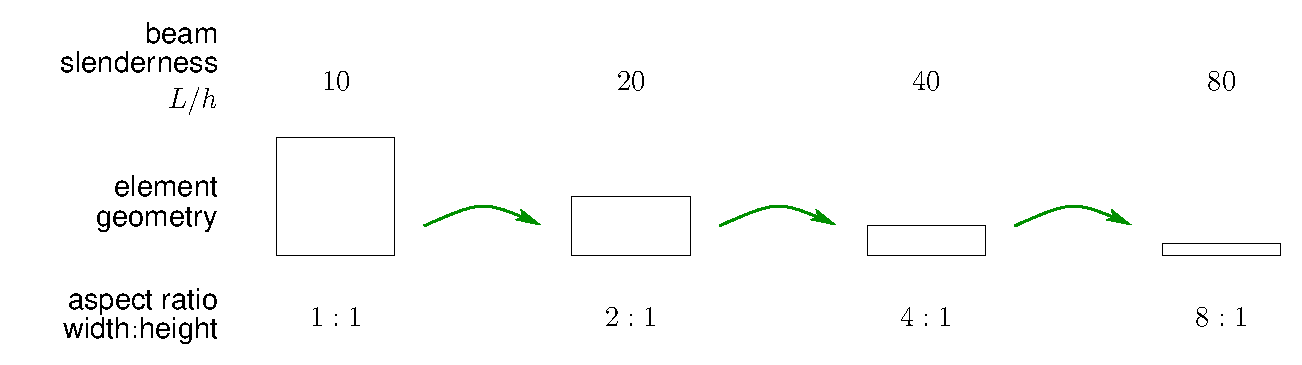
\includegraphics[width=0.8\linewidth]{eps/cantv-evolution-aspect-ratio}
  \end{center}
  \caption{Evolution of element geometry aspect ratio}
  \label{wall1:fig:eas-aspect-ratio-evolution}
\end{figure}

In Figure~\ref{wall1:fig:eas-aspect-ratio-cantilever} the bad influence of
Q1 elements with high aspect ratios can be readily observed.
\begin{figure}[H]
  \begin{center}
    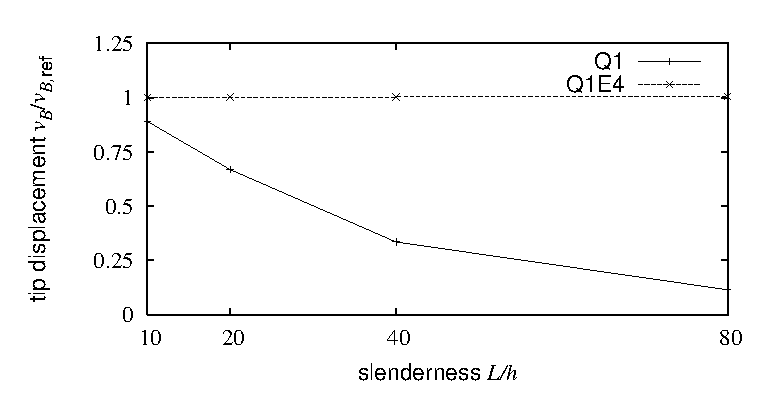
\includegraphics[width=0.8\linewidth]{eps/cantv-tipdispl}
  \end{center}
  \caption{Effect of element aspect ratio }
  \label{wall1:fig:eas-aspect-ratio-cantilever}
\end{figure}
On the ordinate the displacement is scaled by a reference solution computed
with geometrically nonlinear \name{Reissner} beam elements (see for instance
\name{Wriggers}, ``Nichtlineare Finite-Elemente-Methoden'', Springer, 2001). 


\subitempart{\name{Cook}'s cantilever}\\
Figure~\ref{wall1:fig:eas-cook-system} depicts the initial configuration of
\name{Cook}'s cantilever. The 
problem consists of a tapered panel (plane strain, $E=360\unit{GPa}$,
$\nu=0.3$ or $\nu=0.49995$,
$h_1=44\unit{mm}$, $h_2=16\unit{mm}$, $b=48\unit{mm}$) clamped on one end and
subjected to a uniform shearing load $V=100\unit{kN}$ on the opposite end. 
\begin{figure}[H]
  \begin{center}
    \subfigure[undeformed configuration]{
      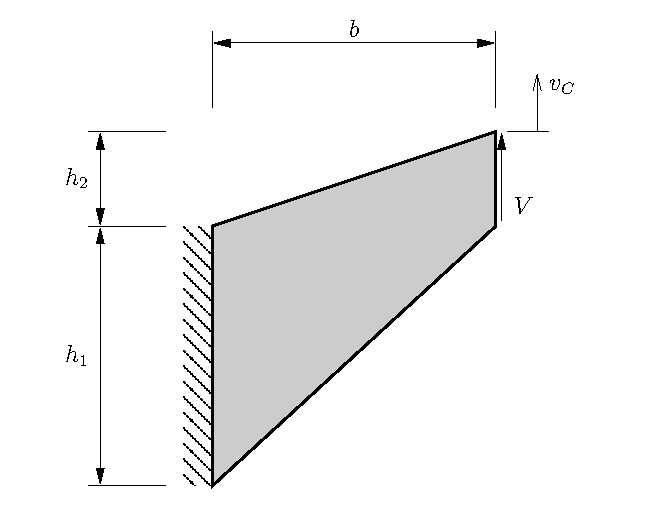
\includegraphics[width=0.3\linewidth]{eps/cook-beam-system}
      \label{wall1:fig:eas-cook-system}}
    \subfigure[undeformed configuration with $16\times16$ Q1 elements]{
      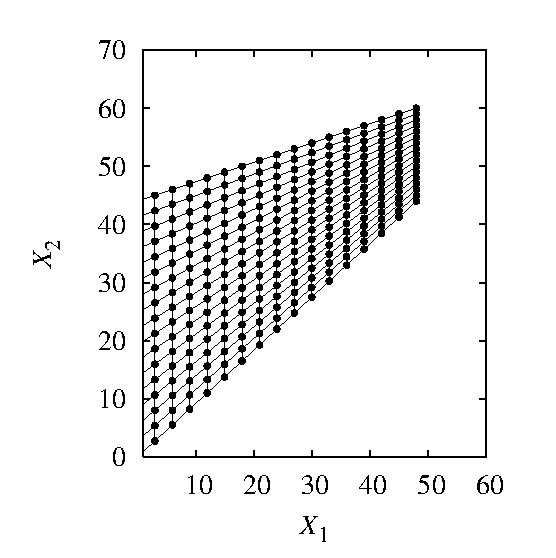
\includegraphics[width=0.3\linewidth]{eps/cook-nu03-initial-d16x16}
      \label{wall1:fig:eas-cook-system-deflected}}
    \subfigure[deformed configuration with $16\times16$ Q1 elements,
      $\nu=0.3$]{
      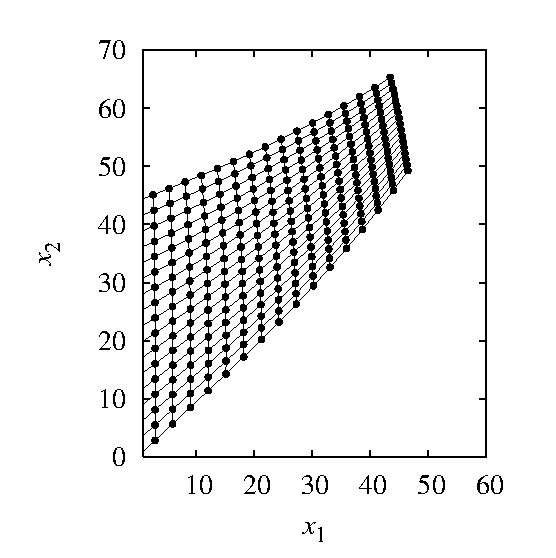
\includegraphics[width=0.3\linewidth]{eps/cook-nu03-deformed-d16x16}
      \label{wall1:fig:eas-cook-system-deflected-2}}
  \end{center}
  \caption{\name{Cook}'s problem}
  \label{wall1:fig:eas-cook-beam}
\end{figure}
Figure~\ref{wall1:fig:eas-cook-convergence-diagrams} includes convergence tests
performed again with the Q1 and Q1E4 
element. The vertical tip displacement $v_C$ is drawn versus the number of
elements per side.
\begin{figure}[H]
  \begin{center}
  \subfigure[Poisson's ratio $\nu=0.3$]{
    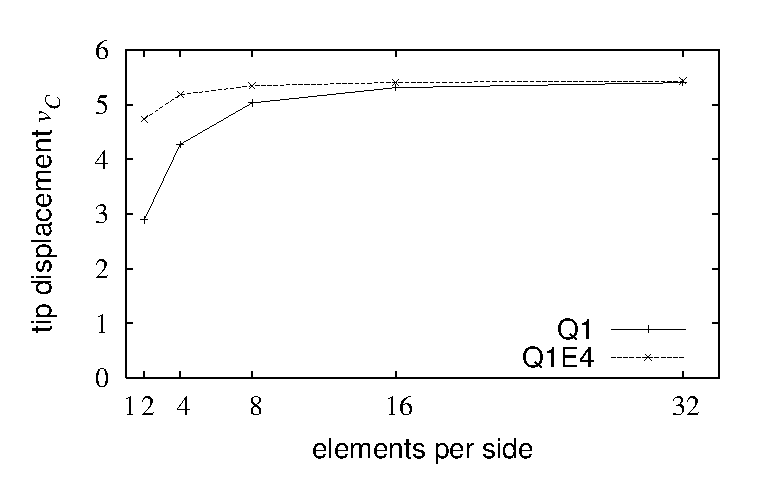
\includegraphics[width=0.45\textwidth]{eps/cook-nu03-tipdispl}
    \label{wall1:fig:eas-cook-convergence-diagram-nu03}}
  \subfigure[Poisson's ratio $\nu=0.49995$]{
    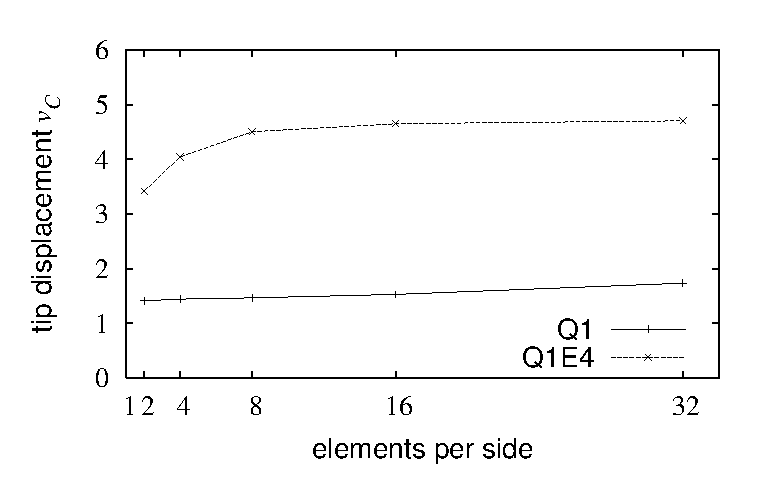
\includegraphics[width=0.45\textwidth]{eps/cook-nu049995-tipdispl}
    \label{wall1:fig:eas-cook-convergence-diagram-nu049995}}
  \end{center}
  \caption{Convergence diagram for tip displacement}
  \label{wall1:fig:eas-cook-convergence-diagrams}
\end{figure}
The convergence diagram is shown for \name{Poisson}'s ratio $\nu=0.3$,
Fig.~\ref{wall1:fig:eas-cook-convergence-diagram-nu03}, and
close to the incompressible limit $\nu=0.49995$,
Fig.~\ref{wall1:fig:eas-cook-convergence-diagram-nu049995}. The Q1 element is
affected by volumetric locking in contrast to the Q1E4 element.

\subitempart{Rotated beam}\\
We consider a beam ($E=40000$, $\nu=0.3$) of length $L=1.0$ and height
$h=0.1$. A transversal 
deflection of $2h$ is imposed at the right end, together with a rigid
rotation with angle $\theta$ around the left bottom vertex. We carry out the
simulations for $\theta=0^\circ, 15^\circ, 
30^\circ, 45^\circ, 60^\circ, 75^\circ, 90^\circ$, and different finite
elements, see Fig.~\ref{wall1:fig:rot-beam-system-displacement}

\begin{figure}[H]
  \begin{center}
    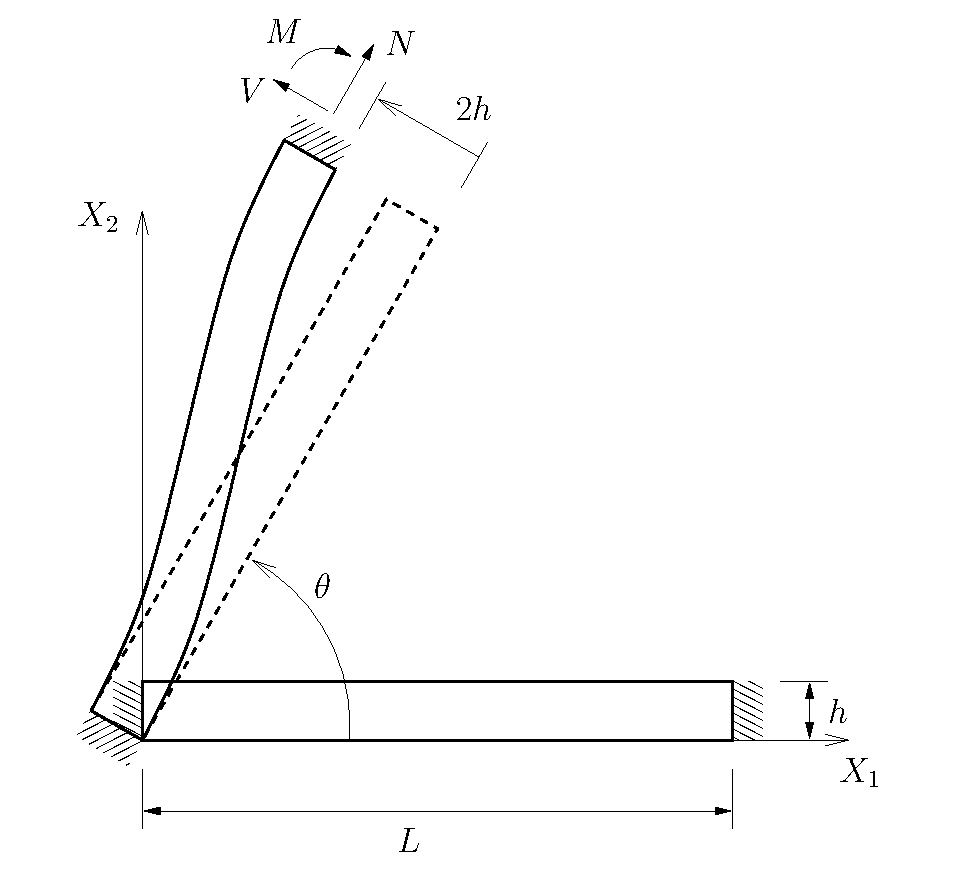
\includegraphics[width=0.4\linewidth]{eps/rot-beam-system}
    \hspace{0ex}
    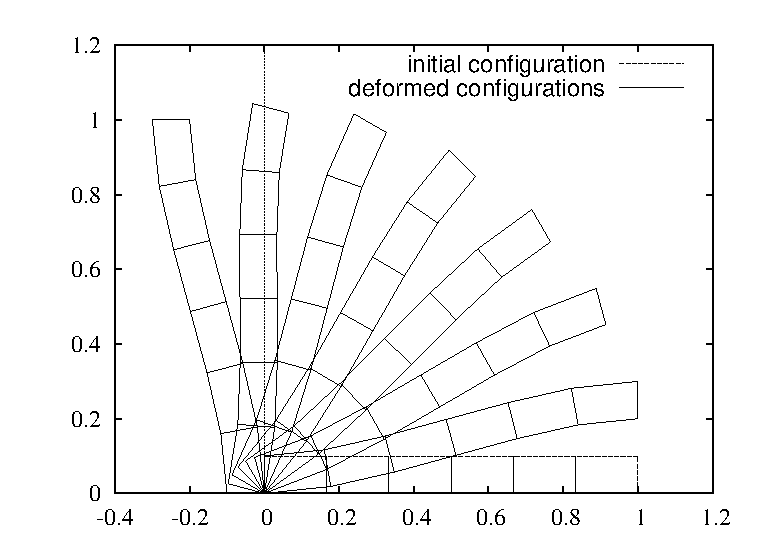
\includegraphics[width=0.55\linewidth]{eps/rot-beam-displacements}
  \end{center}
  \caption{Beam system and deformed states (Q1 and Q1E4 nearly identical)}
  \label{wall1:fig:rot-beam-system-displacement}
\end{figure}

\begin{figure}[H]
  \begin{center}
    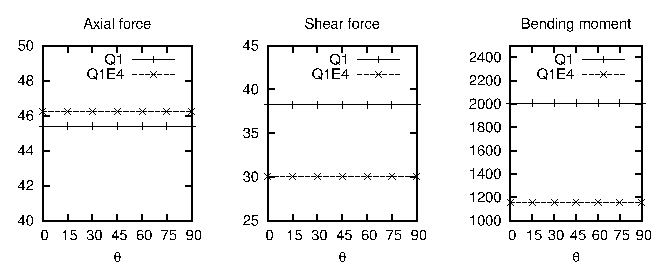
\includegraphics[width=0.8\linewidth]{eps/rot-stress-resultant_b}
  \end{center}
  \caption{Reactions at different angles}
  \label{wall1:fig:rot-stress-resultant}
\end{figure}

Figure~\ref{wall1:fig:rot-stress-resultant} shows the results obtained for the reacting axial, shear and
bending moment in the right support. A frame-indifferent (objective) solution
is characterized by a constant value of these measured quantities with respect
to the superimposed rigid rotation $\theta$. The objectivity is assured of the 
displacement-based Q1 wall element (\cf{} Sec.~\ref{wall1:sec:wall}) and of the
herein presented Q1E4 EAS-element.


%%
%%============================
\subsection{Epilogue}

\begin{itemize}
\item mixed method based on the three-field enhanced strain variational
  principle $\to$ two sets of discrete quantities $\vct{d}^{(e)}$ and
  $\vct{\alpha}^{(e)}$ (stress field is intrinsically satisfied)
\item hybrid approach with discontinuous trial enhanced gradients $\to$ 
  static condensation of element-wise enhanced gradient equations
\item frame-invariant element
\item additional computational effort
\item stability problems $\to$ zero-energy-modes in case of high compression
\item more complicated in 3-dimensions $\to$ current field of research
\item often used in combination with other anti-locking means: red.\@
  integr.\@, ANS, \ldots
\item in general EAS method is used to suppress volumetric locking
\item in general equivalent to the `incompatible modes' approach
\end{itemize}


%%
%%............................
\section{Theory behind the energy-momentum method for the wall elements in
case of \name{de~St.~Venant}--\name{Kirchhoff} material}

This section provides a derivation of the energy-momentum method\footnote{JC
 Simo and N Tarnow, The discrete energy-momentum method, Conserving algorithms
 fro nonlinear elastodynamics, Journal of Applied Mathematics and Physics, 43:757-792, 1992.}
 for the enhanced assumed strain wall element, \cf{}
Sec~\ref{wall1:sec:walleas},  utilising a hybrid 
approach in the case of \name{de~St.~Venant}--\name{Kirchhoff} material.

\subsection{Potential of \name{de St.~Venant}--\name{Kirchhoff} material}
The internal strain energy, or shortly internal energy, of \name{de
St.~Venant}--\name{Kirchhoff} material is a potential $V$ and defined as follows
\begin{equation}
\begin{aligned}
   V 
&  = \frac{1}{2} \int \tns{E} : \tns{S} \, \dd V
&& \text{or}
&  V 
&  = \frac{1}{2} \int \vct{E}^\T \vct{S} \, \dd V
\\
&  = \frac{1}{2} \int \tns{E} : \tns{C}_\VK : \tns{E} \, \dd V
&&
&& = \frac{1}{2} \int \vct{E}^\T \vct{C}_\VK \vct{E} \, \dd V
\end{aligned}
\end{equation}

\subsection{Interal mid-point forces to achieve
energy-momemtum method --- displacement-based element}
An internal mid-point force vector
$\vct{f}_{\Int;m}$ of the purely displacement-based finite element must
satisfy \emph{exactly}
\begin{equation}
   V_{n+1} - V_n
   = \big( \vct{d}_{n+1} - \vct{d}_n \big)^\T \vct{f}_{\Int;m}
\end{equation}
to achieve the energy-momentum method invented by \name{Simo} and
\name{Tarnow}. Here, $n$ denotes the $n$th time step and $m$ a
mid-configuration between $t_n$ and $t_{n+1}$.

Let us now dwell upon the aforementioned potential of
\name{de~St.~Venant}--\name{Kirchhoff} material. We write
\begin{equation}
\begin{aligned}
   V_{n+1} - V_{n}
&  = \frac{1}{2} \int \tns{E}_{n+1} : \tns{C}_\VK : \tns{E}_{n+1} \, \dd V
   - \frac{1}{2} \int \tns{E}_{n} : \tns{C}_\VK : \tns{E}_{n} \, \dd V
\\
&  = \frac{1}{2} \int \big( \tns{E}_{n+1} - \tns{E}_n \big) 
     : \tns{C}_\VK
     : \big( \tns{E}_{n+1} + \tns{E}_n \big) \, \dd V
\\
&  = \int \big( \tns{E}_{n+1} - \tns{E}_n \big) 
     : \frac{\tns{S}_{n+1} + \tns{S}_n}{2} \, \dd V
   \period
\end{aligned}
\end{equation}
The next step denote the \name{Green}--\name{Lagrange} strains
$\tns{E}=\frac{1}{2}(\tns{F}^\T\cdot\tns{F}-\tns{1})$ sin terms of the
deformation gradient $\tns{F}$. We achieve 
\begin{equation}
\begin{aligned}
   V_{n+1} - V_n
&  = \int \frac{1}{2} \big( \tns{F}_{n+1}^\T\cdot\tns{F}_{n+1} - \tns{1}
                            - \tns{F}_{n}^\T\cdot\tns{F}_{n} + \tns{1} \big)
          : \frac{\tns{S}_{n+1} + \tns{S}_n}{2} \, \dd V
\\
&  = \frac{1}{2} \int
     \big( \tns{F}_{n+1}^\T\cdot\tns{F}_{n+1} - \tns{F}_{n}^\T\cdot\tns{F}_{n} \big)
     : \frac{\tns{S}_{n+1} + \tns{S}_n}{2} 
   \, \dd V
   \period
\end{aligned}
\end{equation}
The symmetry of the 2nd \name{Piola}--\name{Kirchhoff} stress tensor $\tns{S}$ permits to
rewrite the last equation
\begin{equation}\label{wall1:eq:pot-diff}
\begin{aligned}
   V_{n+1} - V_n
&  = \frac{1}{2} \int
     \big( \tns{F}_{n+1} - \tns{F}_{n} \big)^\T
     \cdot \big(\tns{F}_{n+1} + \tns{F}_{n} \big)
     : \frac{\tns{S}_{n+1} + \tns{S}_n}{2} 
     \, \dd V
\\
&  = \int \big( \tns{F}_{n+1} - \tns{F}_{n} \big)^\T
     \cdot \frac{\tns{F}_{n+1} + \tns{F}_{n}}{2}
     : \frac{\tns{S}_{n+1} + \tns{S}_n}{2} 
     \, \dd V
     \period
\end{aligned}
\end{equation}
% The latter expression can denoted with the help of the displacement gradient $\tns{H} =
% \tns{F} - \tns{1}$, \ie{}
% \begin{equation}
% \begin{aligned}
%    V_{n+1} - V_n
% &  = \int \big( \tns{1} + \tns{H}_{n+1} - \tns{1} - \tns{H}_{n} \big)^\T
%      \cdot \frac{\tns{F}_{n+1} + \tns{F}_{n}}{2}
%      : \frac{\tns{S}_{n+1} + \tns{S}_n}{2} 
%      \, \dd V
% \\
% &  = \int \big( \tns{H}_{n+1} - \tns{H}_{n} \big)^\T
%      \cdot \frac{\tns{F}_{n+1} + \tns{F}_{n}}{2}
%      : \frac{\tns{S}_{n+1} + \tns{S}_n}{2} 
%      \, \dd V
%      \period
% \end{aligned}
% \end{equation}

We arrive at the point at which we introduce the finite element discretisation
of the deformation gradient, \ie{} in \name{Voigt}-vector form one obtains
\begin{equation}
   \tilvct{F}
   = \tilvct{1} + \mat{B}_\LL \vct{d}
\end{equation}
as presented in Section~\ref{wall1:sec:wall}, in the potential difference
\eqref{wall1:eq:pot-diff}:
\begin{equation}
\begin{aligned}
   V_{n+1}^{(e)} - V_n^{(e)}
&  = \int_{\Omega^{(e)}} \big( \tilvct{F}_{n+1} - \tilvct{F}_{n} \big)^\T
     \frac{\barmat{F}_{n+1} + \barmat{F}_{n}}{2}
     \frac{\vct{S}_{n+1} + \vct{S}_n}{2} 
     \, \dd V
\\
&  = \int_{\Omega^{(e)}}
     \big( \tilvct{1} + \mat{B}_\LL \vct{d}_{n+1} 
           - \tilvct{1} - \mat{B}_\LL \vct{d}_n \big)
     \frac{\barmat{F}_{n+1} + \barmat{F}_{n}}{2}
     \frac{\vct{S}_{n+1} + \vct{S}_n}{2} 
     \, \dd V
\\
&  = \big( \vct{d}_{n+1} - \vct{d}_n \big)
     \underbrace{\int_{\Omega^{(e)}}
     \mat{B}_\LL \frac{\barmat{F}_{n+1} + \barmat{F}_{n}}{2}
     \frac{\vct{S}_{n+1} + \vct{S}_n}{2} 
     \, \dd V}_{\displaystyle\vct{f}_{\Int;m}}
     \period
\end{aligned}
\end{equation}
The energy-momentum conserving internal mid-force vector for \name{de
St.~Venant}--\name{Kirchhoff} material is thus
\begin{equation}\label{wall1:eq:mid-internal-pure-disp-vkmat}
   \vct{f}_{\Int;m}
   = \int_{\Omega^{(e)}}
     \mat{B}_\LL \underbrace{\frac{\barmat{F}_{n+1} + \barmat{F}_{n}}{2}}_{\barmat{F}_m}
     \underbrace{\frac{\vct{S}_{n+1} + \vct{S}_n}{2}}_{\vct{S}_m}
     \, \dd V
\end{equation}
with the mid-deformation gradient $\barmat{F}_m=\frac{1}{2}(\barmat{F}_{n+1} +
\barmat{F}_{n})$ (denoted as \name{Voigt}-matrix) and 2nd
\name{Piola}--\name{Kirchhoff} mid-stress $\vct{S}_m =
\frac{1}{2}(\vct{S}_{n+1} + \vct{S}_n)=\mat{C}_\VK\big(\frac{1}{2}(\vct{E}_{n+1} + \vct{E}_n)\big)$ (denoted as \name{Voigt}-vector).

\subsubsection{Generalised energy-momentum method}
The generalised energy-momentum method\footnote{D Kuhl and MA Crisfield,
Energy-conserving and decaying algorithms in non-linear structural dynamics,
International Journal for Numerical Methods in Engineering, 45(5):569-599,
1999.} modifies the evaluation of the mid-gradient and -stress in
\eqref{wall1:eq:mid-internal-pure-disp-vkmat}. It is defined as
\begin{equation}
\begin{aligned}
   \vct{f}_{\Int;m}
&  = \int_{\Omega^{(e)}}
     \mat{B}_\LL
     {\barmat{F}_m}
     {\vct{S}_m}
     \, \dd V
&& \text{with}
&  \barmat{F}_m
&  = (1-\alpha_f) \barmat{F}_{n+1} + \alpha_f \barmat{F}_n
&& \text{and}
&&  \alpha\in[0,1)
   \comma
\\
&
&&
&  \vct{S}_m
&  = \mat{C}_\VK \big( (1-\alpha_f+\xi)\vct{E}_{n+1} +
(\alpha_f-\xi)\vct{E}_{n} \big)
&&
&& \xi\in[0,1)
   \period
\end{aligned}
\end{equation}
Obviously, this method conserves energy only if $\alpha_f=1/2$ and $\xi=0$.
  

\subsubsection{Stiffness matrix}
The stiffness matrix $\mat{k}^{(e)}_m$ is readily computed as
\begin{equation}
\begin{aligned}
   \mat{k}_m
&  = \frac{\pd \vct{f}_{\Int;m}}{\pd \vct{d}_{n+1}}
\\
&  = \int_{\Omega^{(e)}}
   \mat{B}_\LL \barmat{F}_m \vct{S}_{m,\vct{d}}
   \, \dd V
   + \int_{\Omega^{(e)}}
   \mat{B}_\LL \barmat{F}_{m,\vct{d}} \vct{S}_{m}
   \, \dd V
\\
&  = \int_{\Omega^{(e)}}
   \mat{B}_\LL \barmat{F}_m (1-\alpha_f+\xi)\left.\vct{S}_{,\vct{d}}\right|_{n+1}
   \, \dd V
   + \int_{\Omega^{(e)}}
   \mat{B}_\LL (1-\alpha_f)\left.\barmat{F}_{,\vct{d}}\right|_{n+1} \vct{S}_{m}
   \, \dd V
\\
&  = \underbrace{\int_{\Omega^{(e)}}
   \mat{B}_\LL \barmat{F}_m (1-\alpha_f+\xi) \mat{C}_\VK \barmat{F}_{n+1}^\T \mat{B}_\LL
   \, \dd V}_{\mat{k}_{\ela\ini;m}}
   + \underbrace{\int_{\Omega^{(e)}}
   \mat{B}_\LL \barmat{S}_{m} (1-\alpha_f)\mat{B}_\LL
   \, \dd V}_{\mat{k}_{\geo;m}}
   \period
\end{aligned}
\end{equation}

\subsection{Interal mid-point forces to achieve
energy-momemtum method --- EAS-displacement-based element}
Similarly in case of the mixed element approach based on displacement and EAS
parameters, the internal energy difference must be recovered exactly by
\begin{equation}
   V_{n+1} - V_n
   = \big( \vct{d}_{n+1} - \vct{d}_n \big)^\T \vct{f}_{\Int;m}
   + \big( \vct{\alpha}_{n+1} - \vct{\alpha}_n \big)^\T
   \underbrace{\vct{s}_m}_{\to \vct{0}}
   \comma
\end{equation}
in which $\vct{f}_{\Int;m}$ is once more the internal mid-force vector and
$\vct{s}_m$ the mid-point enhanced assumed strain constraint, \cf{}
\eqref{wall1:eq:eas-constraint-vector}. 

%%% Local Variables: 
%%% mode: latex
%%% TeX-master: "nfem"
%%% End: 
